%!TEX root = ../../thesis.tex

\Section~\ref{sec:signature} outlined the basic experimental signature of the search as 
two oppositely charged leptons and significant \met. Thus, the initial stages of the 
event selection are tasked with finding this signature. Subsequent criteria, or 
\textit{cuts}, target specific backgrounds. Their aim is improve the analysis sensitivity 
by suppressing backgrounds whilst retaining a sufficient number of signal events.



\subsection{Data quality}
\label{sec:selection:quality}

The \pp dataset (see \Section~\ref{sec:dataset:dataset}) is hierarchically split into 
\textit{periods} of broadly consistent beam conditions, \textit{runs} typically 
corresponding to LHC fills, and \textit{luminosity blocks} of \about 2~minutes where the 
instantaneous luminosity is approximately constant. Luminosity blocks are included in the 
analysis if the detector was operating sufficiently for the recorded data to be 
considered `good for physics' (see \Figure~\ref{fig:dataset:lumi}).\footnote{
	ATLAS good runs list: \texttt{data12\symbol{95}8TeV.periodAllYear\symbol{95}DetStatus-v61-pro14-02\symbol{95}DQDefects-00-01
	-00\symbol{95}PHYS\symbol{95}StandardGRL\symbol{95}All\symbol{95}Good.xml}
} 
For the 2012 dataset, this corresponds to a total integrated luminosity of 
\unit{20.3}{\invfb}.

Individual events are also vetoed if certain data quality criteria are failed by:
\begin{itemize}[noitemsep,nolistsep]
	\item a noise burst in the LAr calorimeter,
	\item data corruption caused by a restart of the synchronisation system,
	\item a \textit{looser} jet is reconstructed with \unit{$\pt > 20$}{\GeV} (indicative 
	of an HCal spike),
	\item a jet is reconstructed near a `hot' HCal tile (1st -- 8th May 2012 only).
\end{itemize}
A further quality criterion requires that the primary vertex considered as the hard 
scatter (that with the highest $\sum p_{\text{T}}^2$) must be associated with at least 
three tracks. This reduces the cosmic ray background to negligible levels.



\subsection{Trigger}
\label{sec:selection:trigger}

It is infeasible to record all events in the \unit{20.3}{\invfb} dataset; ATLAS instead 
employs a trigger system to identify and record interesting events (see 
\Section~\ref{sec:atlas:trig}). In the \HWWlvlv search it is natural to trigger on 
high-\pt leptons, using algorithms similar to, though less sophisticated than, those in 
\Section~\ref{sec:objects:electrons} and \Section~\ref{sec:objects:muons}.

A trigger is characterised by its efficiency versus \pt curve (though it also depends on 
$\eta$), which has a turn-on followed by a plateau, as shown in 
\Figure~\ref{fig:sel:trig_eff}. It is preferable to operate on the plateau, where the 
efficiency is more stable. To maximise the signal yield, it is desirable to use a trigger 
with a lower turn-on \pt. However, increased backgrounds and limitations to trigger 
latency and bandwidth require a compromise to be found. The lowest unprescaled\footnote{
	A \textit{prescaled} trigger reduces the turn-on \pt by recording only 1 in $N$ 
	events passing the trigger, and weighting such events by a factor $N$. In doing so, 
	some statistical power is lost.
}
single lepton triggers available in 2012 had nominal \pt thresholds of \unit{24}{\GeV}. 
Fortunately, it is possible to recover trigger efficiency at low-\pt by using dilepton 
triggers, because the backgrounds are much smaller.

\begin{figure}
	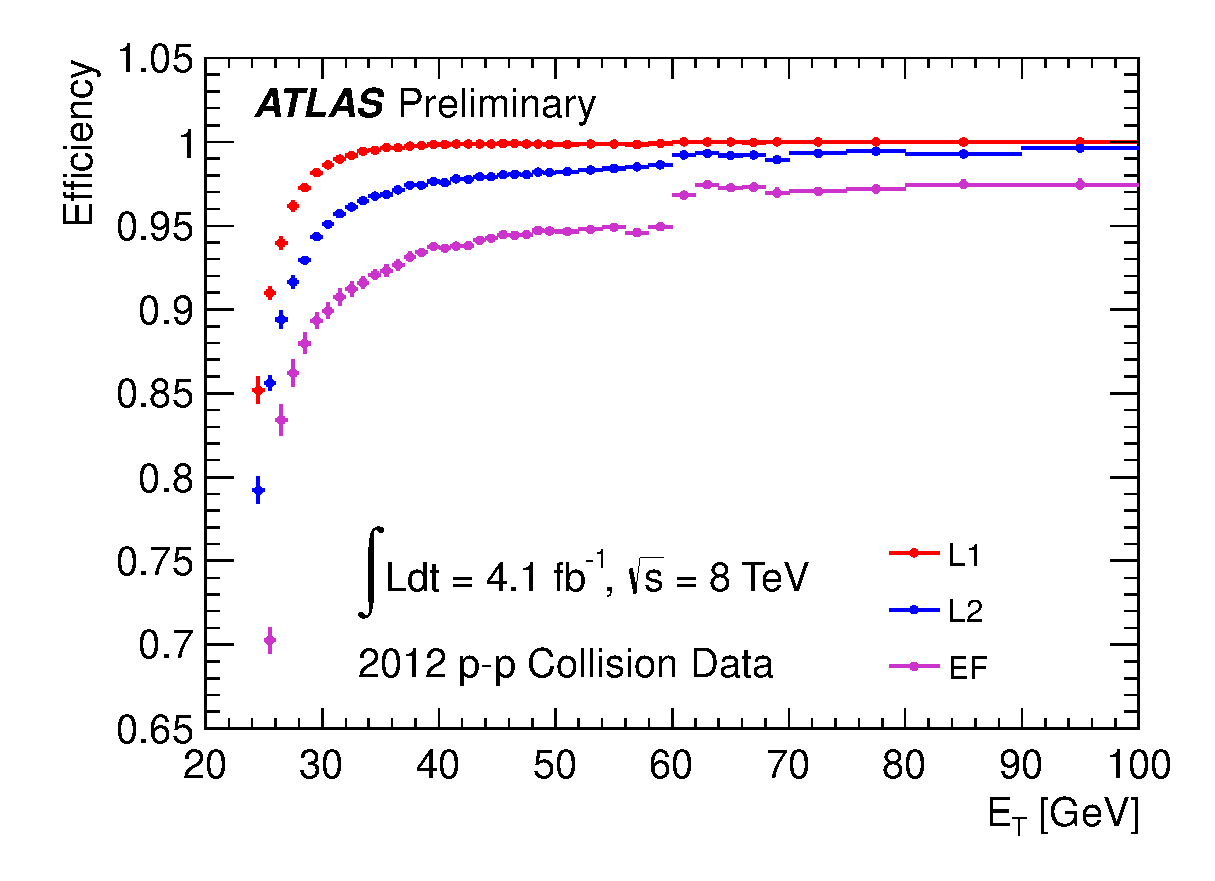
\includegraphics[width=0.495\textwidth]{tex/selection/trigger_eff_el}
	\hfill
	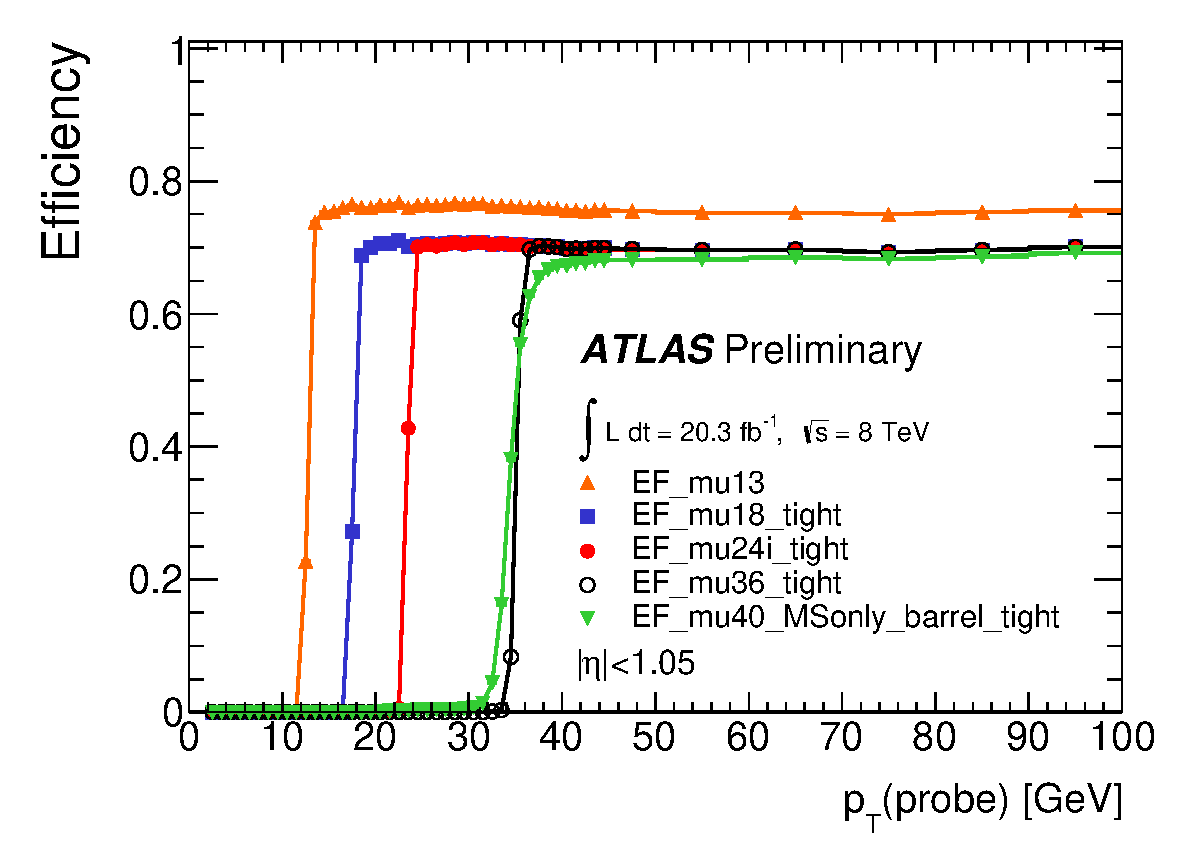
\includegraphics[width=0.495\textwidth]{tex/selection/trigger_eff_mu}
	\caption{Efficiencies of the single lepton triggers for electrons with respect to 
	offline \textit{medium} identification (left) and muons with respect to offline 
	reconstruction (right).}
	\label{fig:sel:trig_eff}
\end{figure}

Events are required to pass at least one trigger listed in \Table~\ref{tab:sel:triggers}. 
The single lepton triggers include a tighter low-\pt trigger and a looser high-\pt 
trigger in order to maximise the efficiency. Dilepton triggers are then used to increase 
the efficiency during the turn-on of the single lepton triggers. Together, these triggers 
support a \pt threshold of \unit{22}{\GeV} on the leading lepton (in the 
offline analysis), whilst operating on the plateau.

\begin{table}
	\begin{tabular}{lllcl}
		\multirow{2}{2.5cm}{Single lepton triggers} & \Pe  & \verb|EF_e24vhi_medium1| & or & \verb|EF_e60_medium1| \\
		& \Pmu & \verb|EF_mu24i_tight| & or & \verb|EF_mu36_tight|  \\
		\hline
		\multirow{3}{2.5cm}{Dilepton triggers} & \HepProcess{\Pe\Pe} & \verb|EF_2e12Tvh_loose1| & or & \verb|EF_2e12Tvh_loose1_L2StarB| \\
		& \HepProcess{\Pmu\Pmu} & \multicolumn{3}{l}{\texttt{EF\symbol{95}mu18\symbol{95}tight\symbol{95}mu8\symbol{95}EFFS}} \\
		& \HepProcess{\Pe\Pmu}  & \multicolumn{3}{l}{\texttt{EF\symbol{95}e12Tvh\symbol{95}medium1\symbol{95}mu8}} \\
	\end{tabular}
	\caption{Employed trigger names. \texttt{EF} refers to event filter, \texttt{e} is an 
	electron, \texttt{mu} is a muon, the following number is the \pt threshold, 
	\texttt{vh} indicates calorimeter isolation, \texttt{i} indicates track isolation, 
	and \texttt{tight}, \texttt{medium} or \texttt{loose} is the identification. Other 
	parts relate to the trigger chain. Criteria are looser than those applied 
	offline.}
	\label{tab:sel:triggers}
\end{table}

Trigger efficiencies are measured via tag-and-probe of 
\HepProcess{\PZ \HepTo \Plepton\Plepton} events, where the tag and probe have both 
passed the offline lepton selection and the tag has successfully matched to a triggered 
lepton object. For example, single lepton trigger efficiencies are displayed in 
\Figure~\ref{fig:sel:trig_eff}. Comparison with MC yields efficiency scale factors.

Additionally, events are required to have at least one lepton passing the offline 
reconstruction that is matched within $\Delta R < 0.15$ of a triggered lepton object.
Single lepton triggers are matched to offline leptons with $\pt > \unit{25}{\GeV}$. On 
the other hand, dilepton triggers comprise two triggered objects: \texttt{mu8} is matched 
to offline muons with $\pt > \unit{10}{\GeV}$, \texttt{mu18} is matched to offline muons 
with $\pt > \unit{20}{\GeV}$, and \texttt{e12} is matched to offline electrons with 
$\pt > \unit{15}{\GeV}$.



\subsection{Pre-selection of dilepton + \met signature}
\label{sec:selection:presel}

Following the trigger selection, events are required to have two oppositely charged 
leptons passing the offline selection (see \Section~\ref{sec:objects}). The lepton with 
the highest \pt, called the \textit{leading lepton}, must have 
\unit{$\ptleadlep > 22$}{\GeV} in order to operate on the trigger plateau. The 
\textit{subleading lepton} must have \unit{$\ptsubleadlep > 10$}{\GeV}, as specified in 
\Section~\ref{sec:objects}. Events containing a third lepton are vetoed in order to 
reject backgrounds with three or more leptons in the final state, such as \WZ production.

At this point, it is possible to split the dilepton final state into four channels 
according to the flavours of the two leptons: \eech, \mmch, \emch, \mech (where the first 
flavour is that of the leading lepton). This is very useful because the background 
compositions of the channels are dramatically different. For example, the \DY background 
is much larger in the same flavour channels (\eech/\mmch) than the different flavour 
channels (\emch/\mech).

Low mass hadronic resonances with dileptonic decays (\eg \PJpsi) are removed from the 
\eech/\mmch channels by requiring the mass of the dilepton system 
\unit{$\mll > 12$}{\GeV}. 
This also greatly suppresses the low mass \DY background. For the \emch/\mech channels, 
a cut of \unit{$\mll > 10$}{\GeV} suppresses leptons from heavy flavour decays. The 
\eech/\mmch channels are hugely dominated by the \DY background (see 
\Figure~\ref{fig:sel:mll}), but most of these events can be rejected by 
vetoing a window around the \PZ mass, \unit{$\mods{\mll - \mZ} > 15$}{\GeV}.

\begin{figure}
	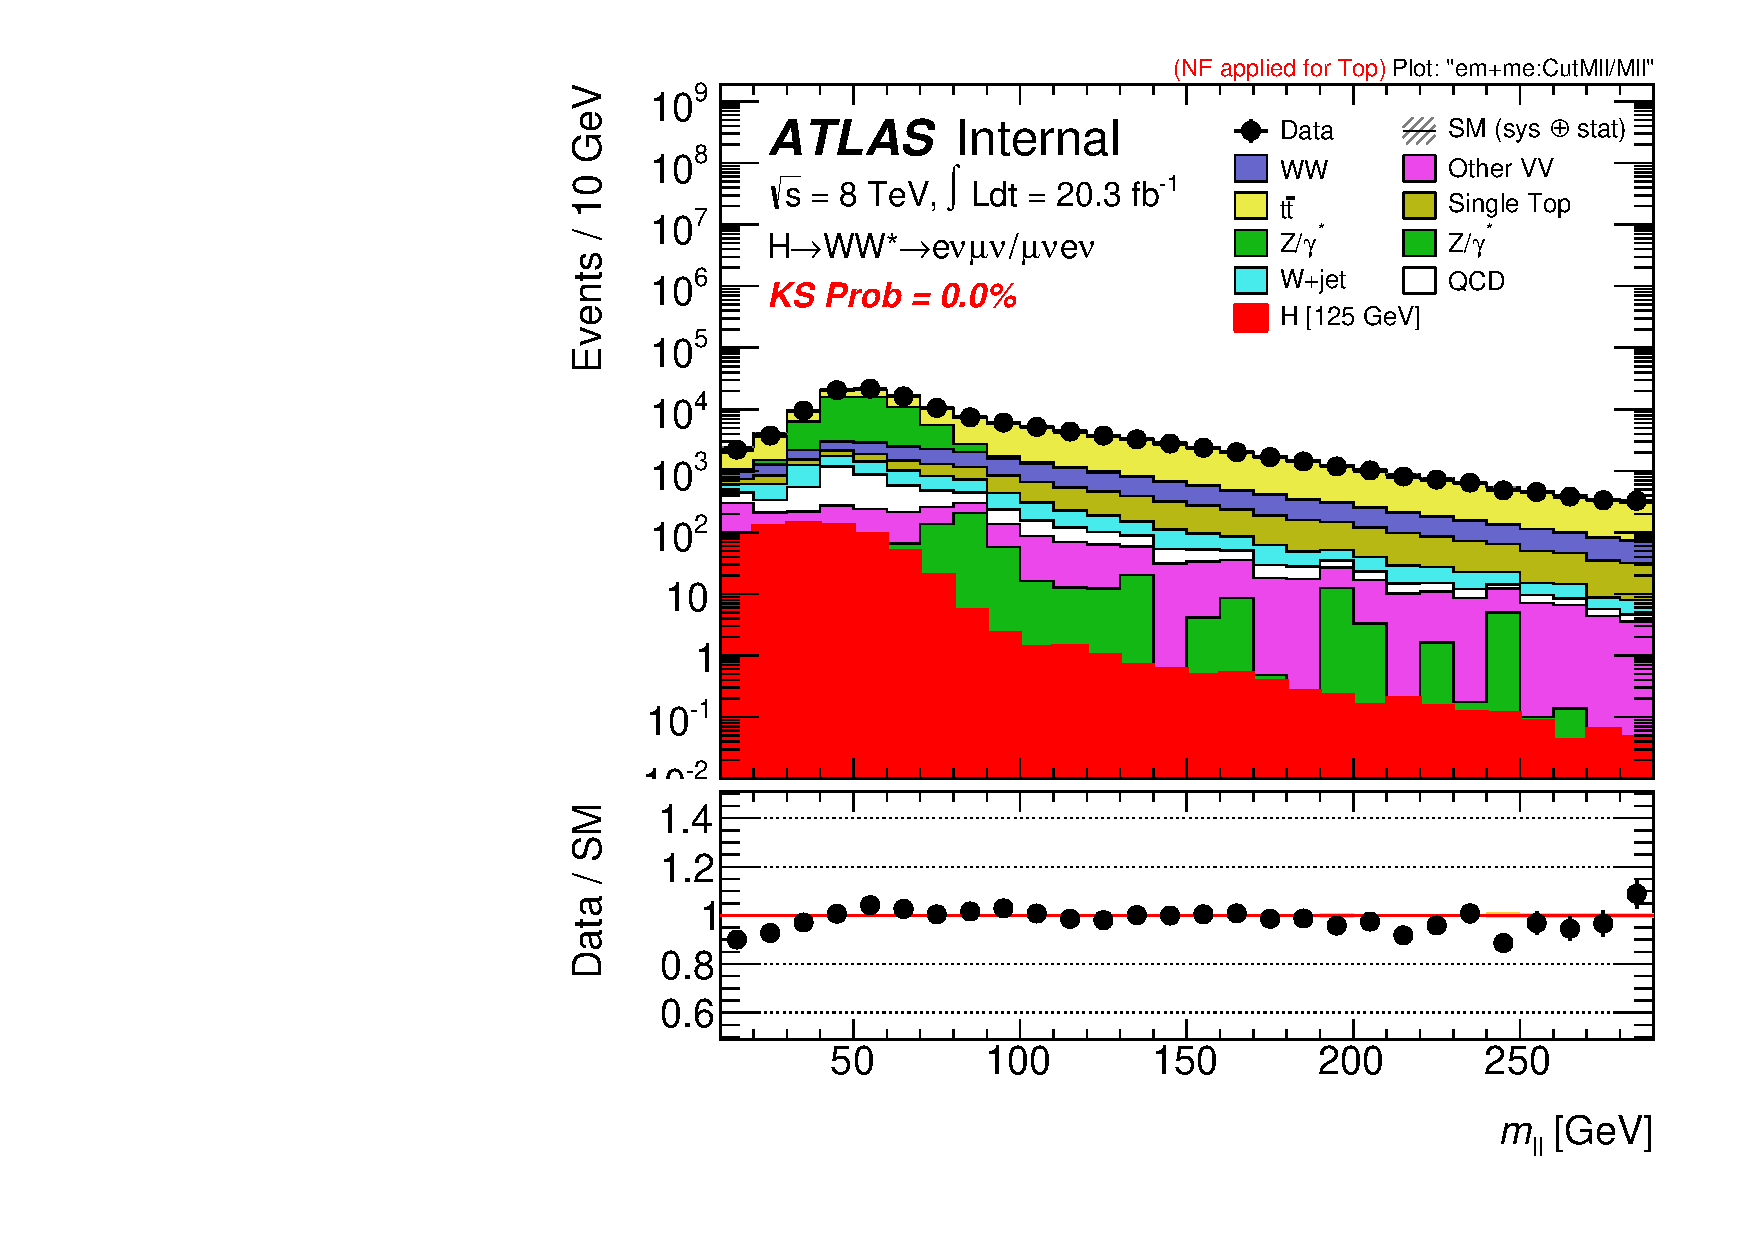
\includegraphics[width=0.495\textwidth]{tex/selection/emme_CutMll_Mll_mh125_log}
	\hfill
	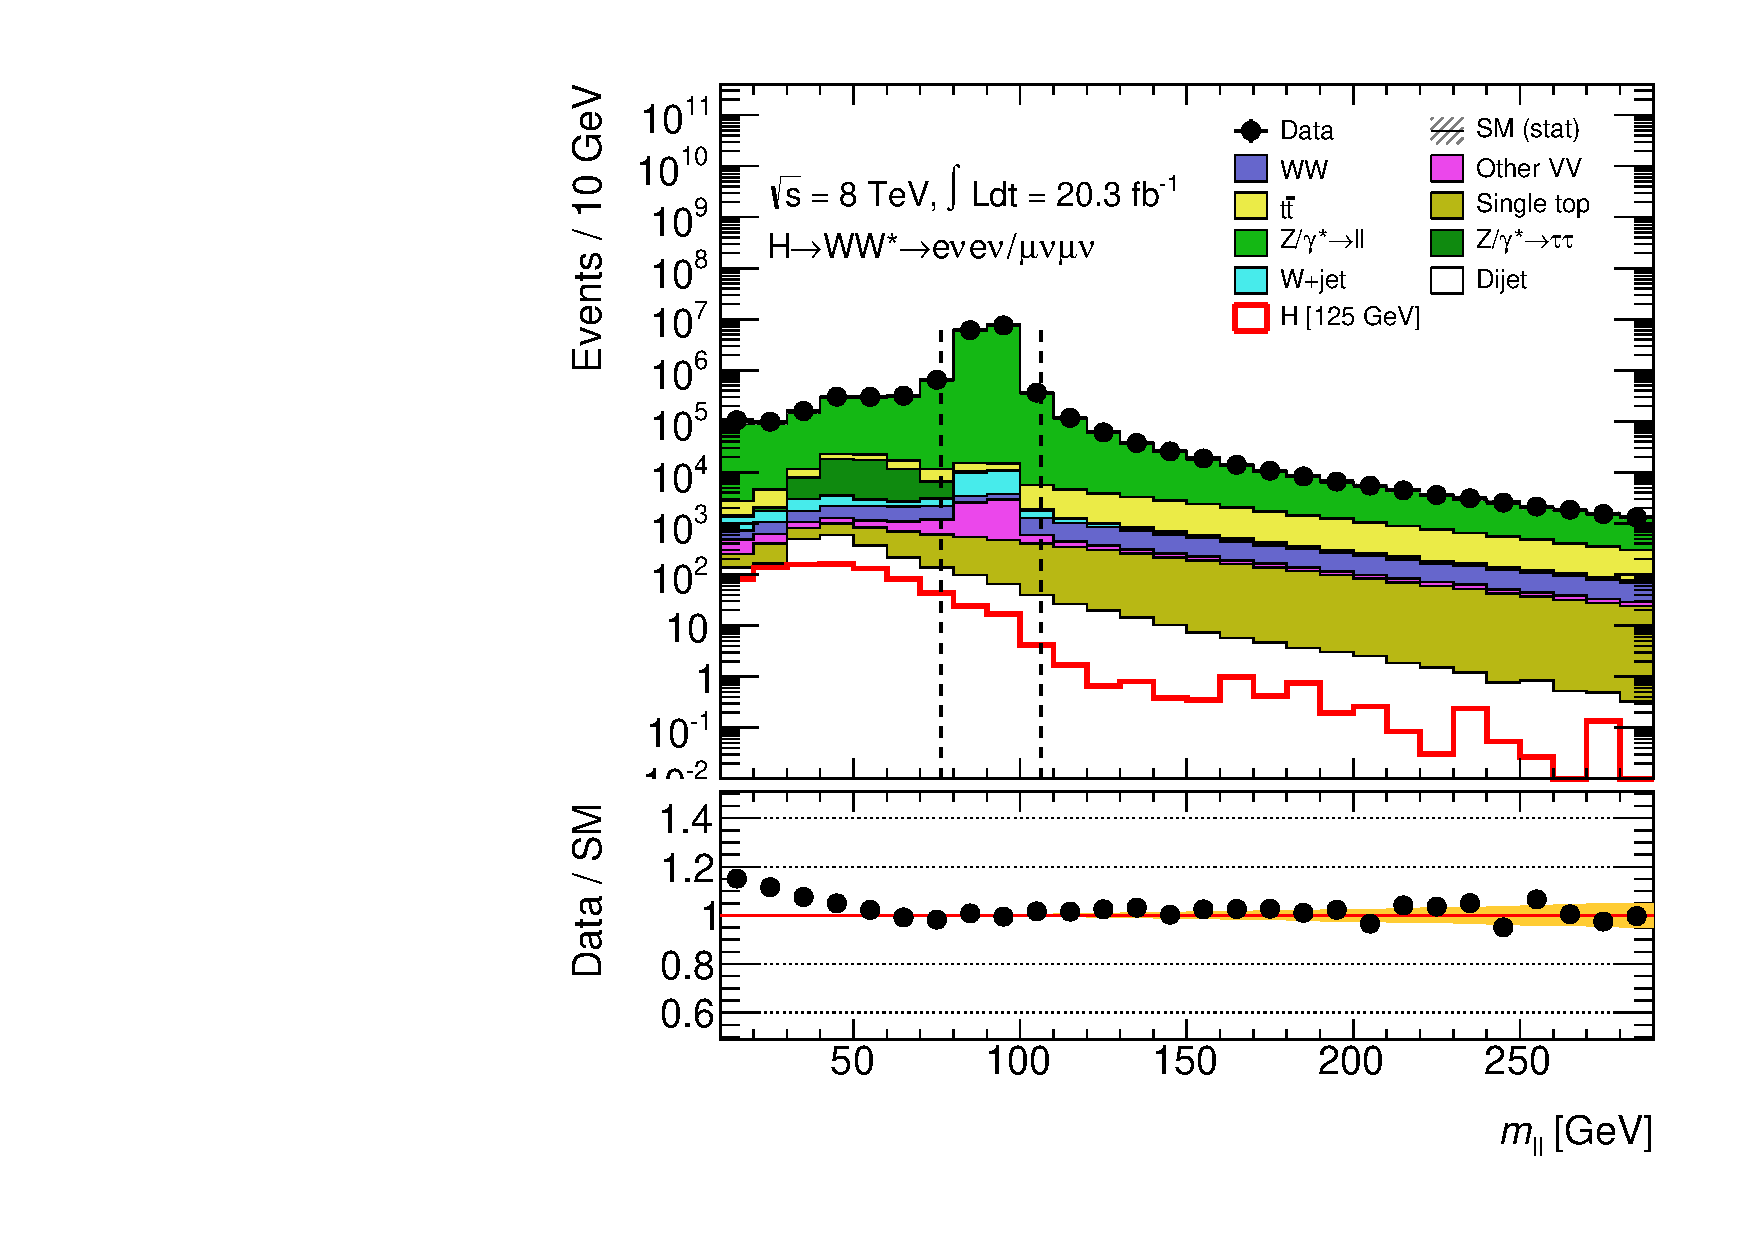
\includegraphics[width=0.495\textwidth]{tex/selection/eemm_CutMll_Mll_mh125_log}
	\caption{Dilepton mass distribution directly preceding the \PZ mass veto, in the 
	\emch/\mech (left) and \eech/\mmch (right) channels.}
	\label{fig:sel:mll}
\end{figure}

\begin{figure}
	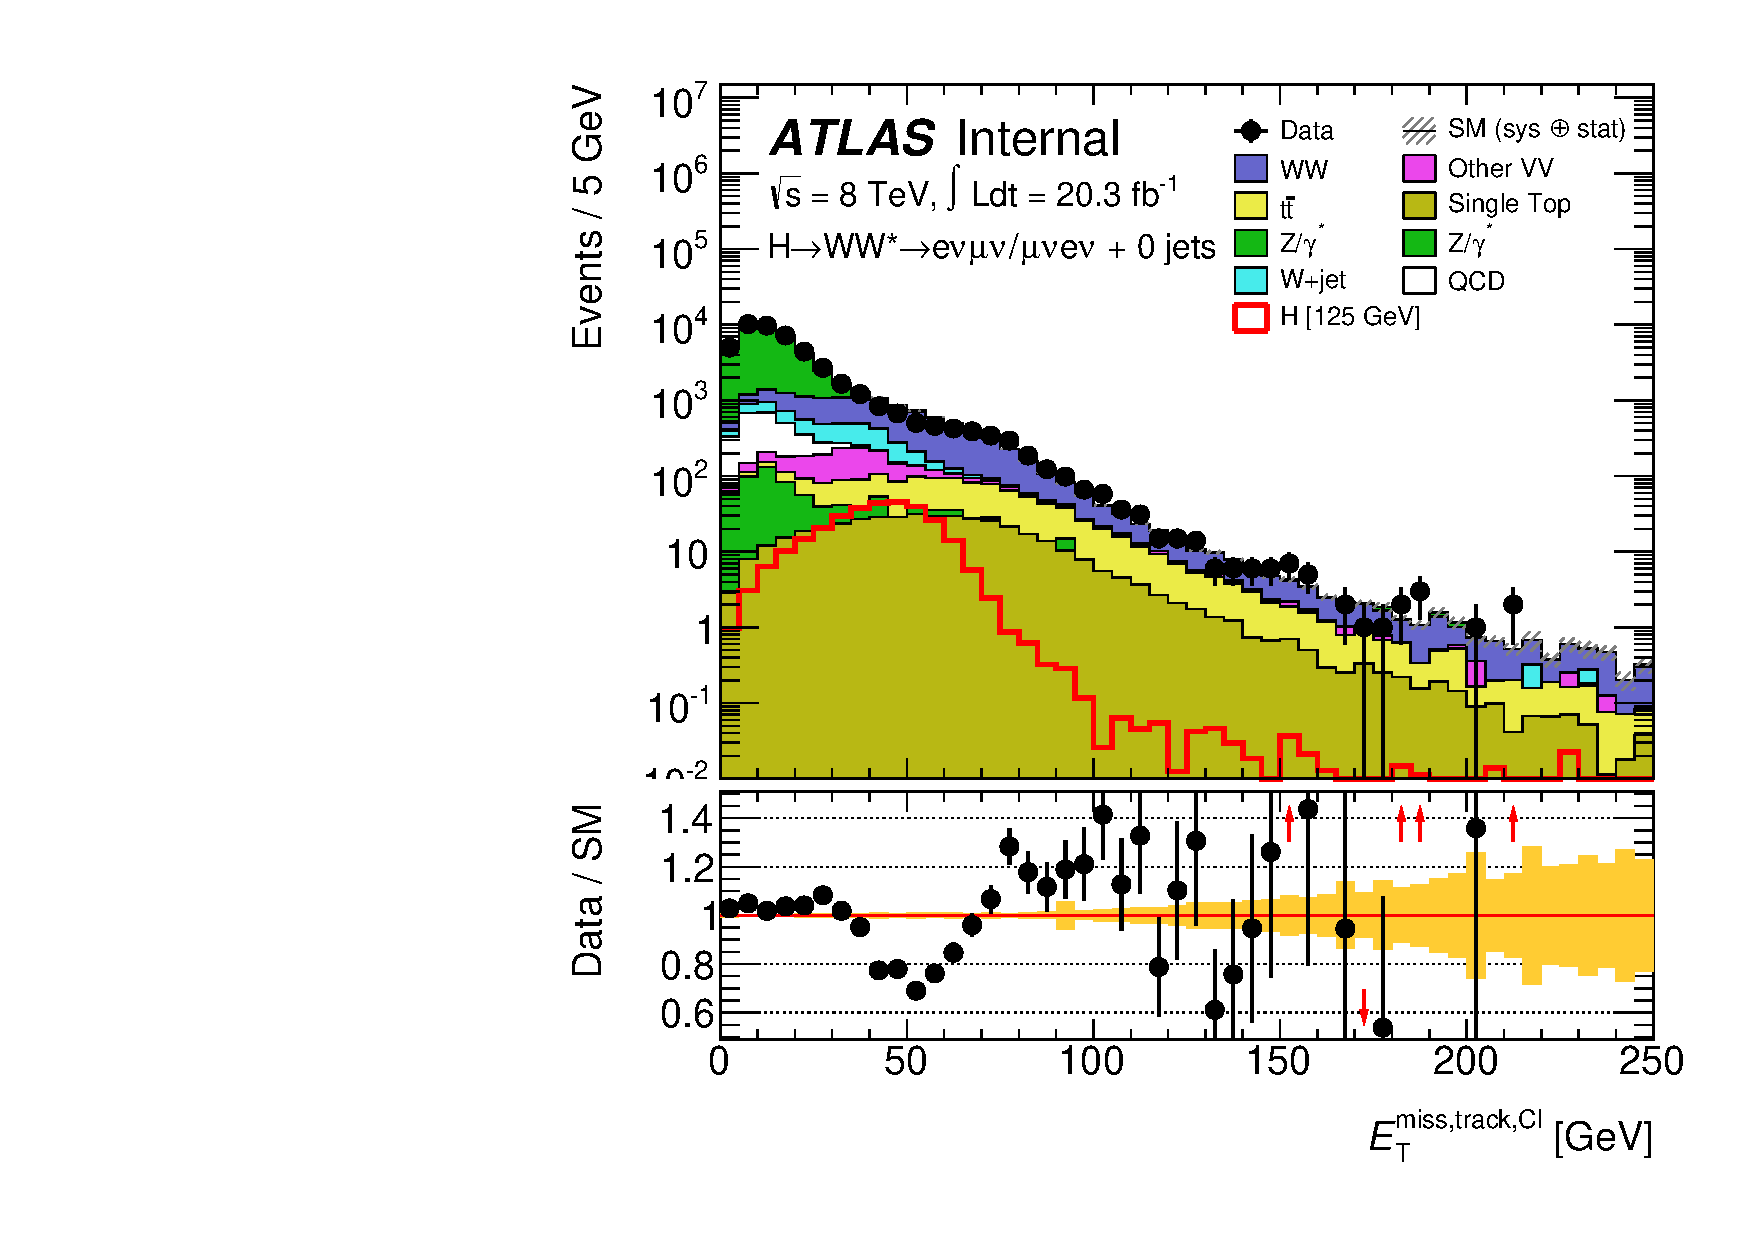
\includegraphics[width=0.495\textwidth]{tex/selection/emme_CutZVeto_0jet_MET_TrackHWW_Clj_mh125_log}
	\hfill
	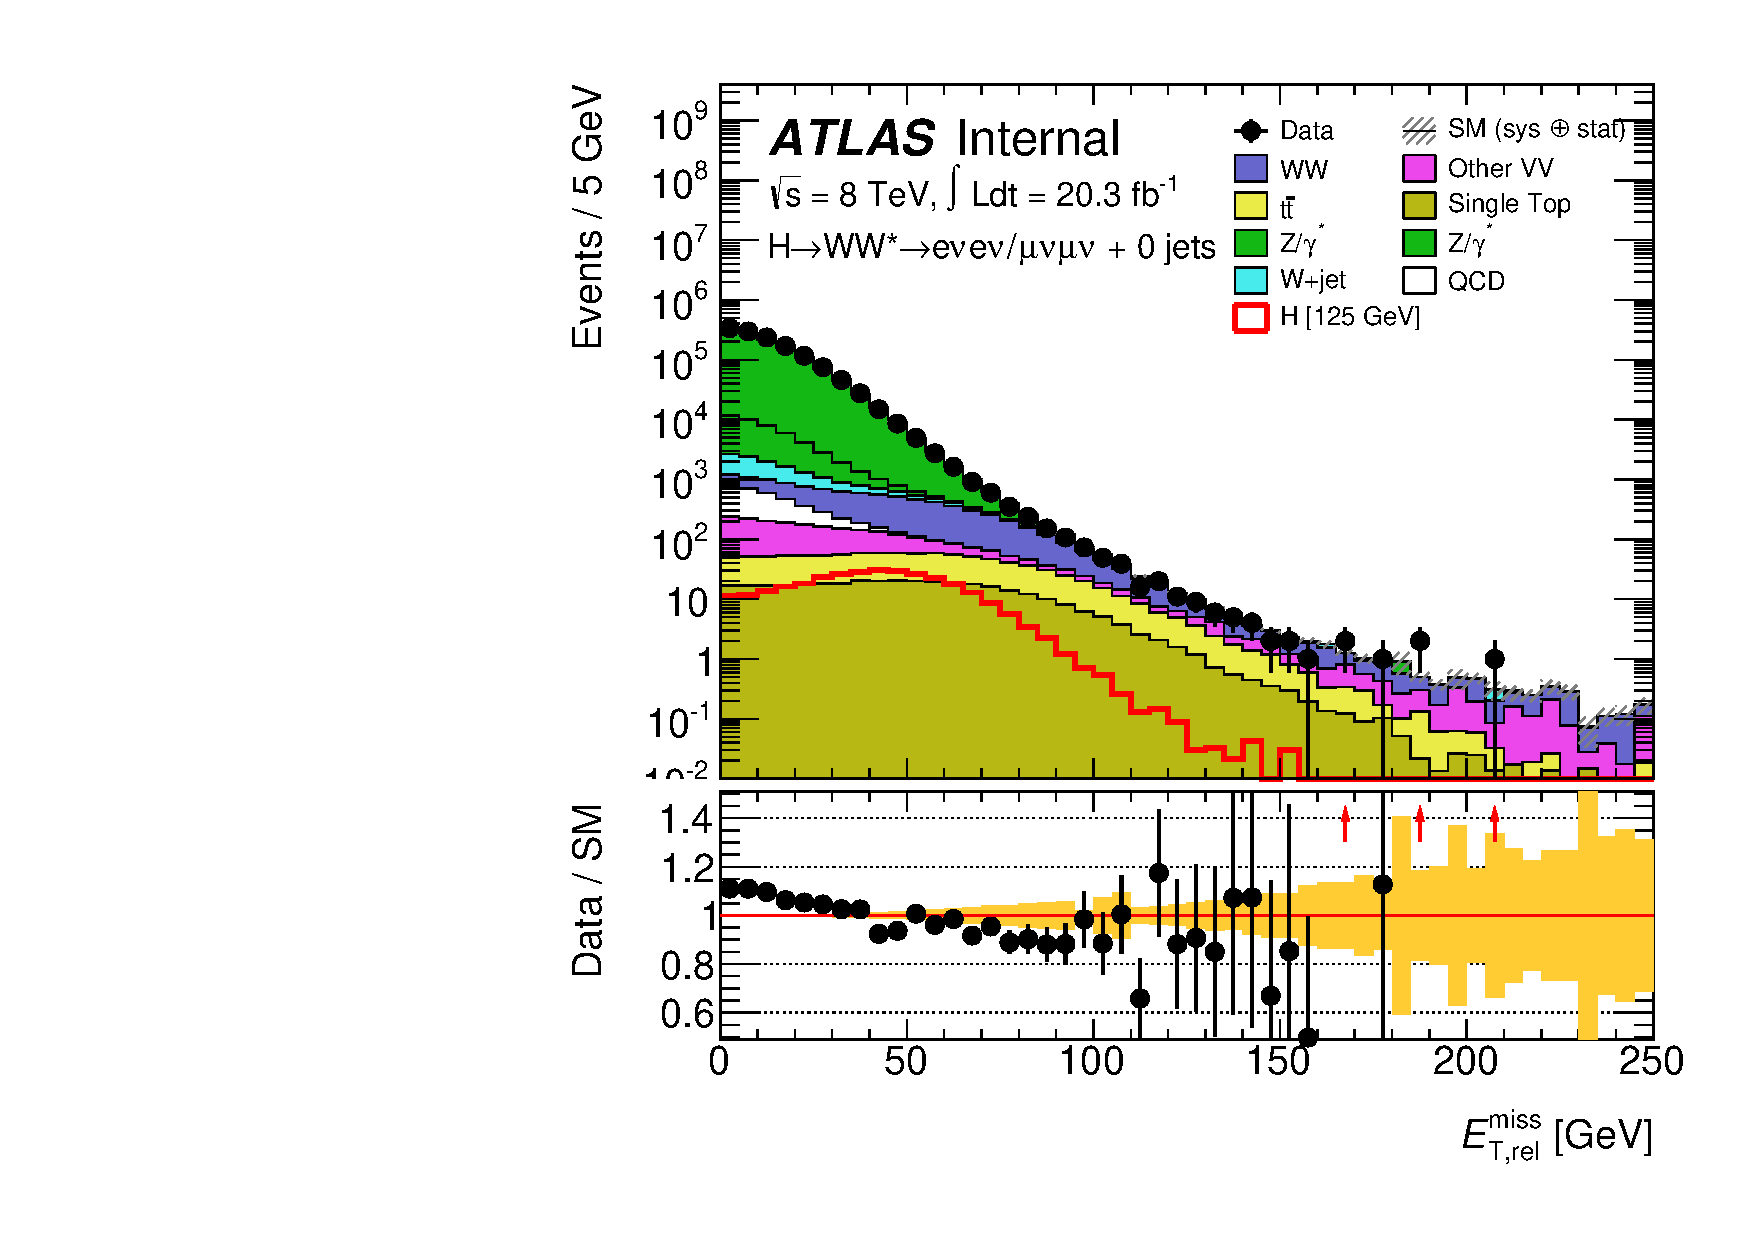
\includegraphics[width=0.495\textwidth]{tex/selection/eemm_CutZVeto_0jet_METRel_mh125_log}
	\\
	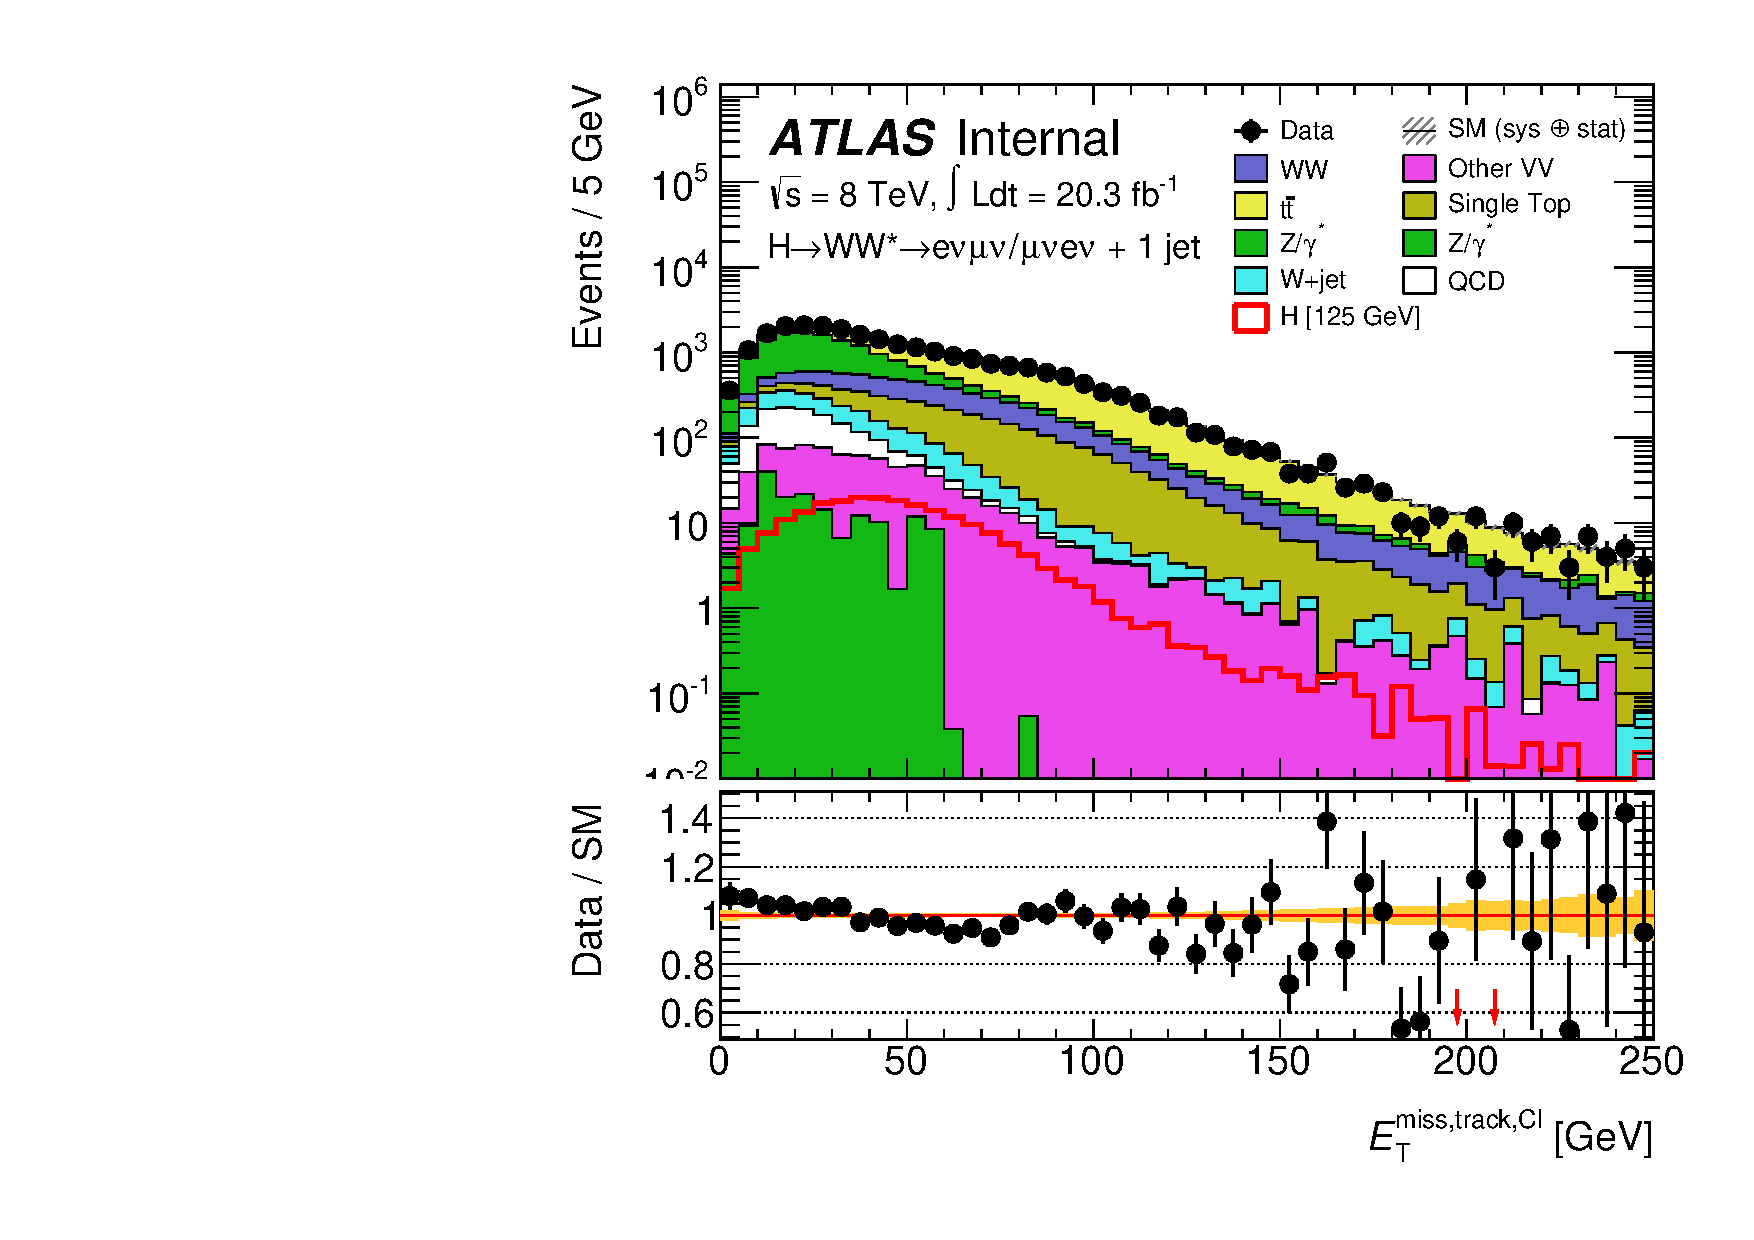
\includegraphics[width=0.495\textwidth]{tex/selection/emme_CutZVeto_1jet_MET_TrackHWW_Clj_mh125_log}
	\hfill
	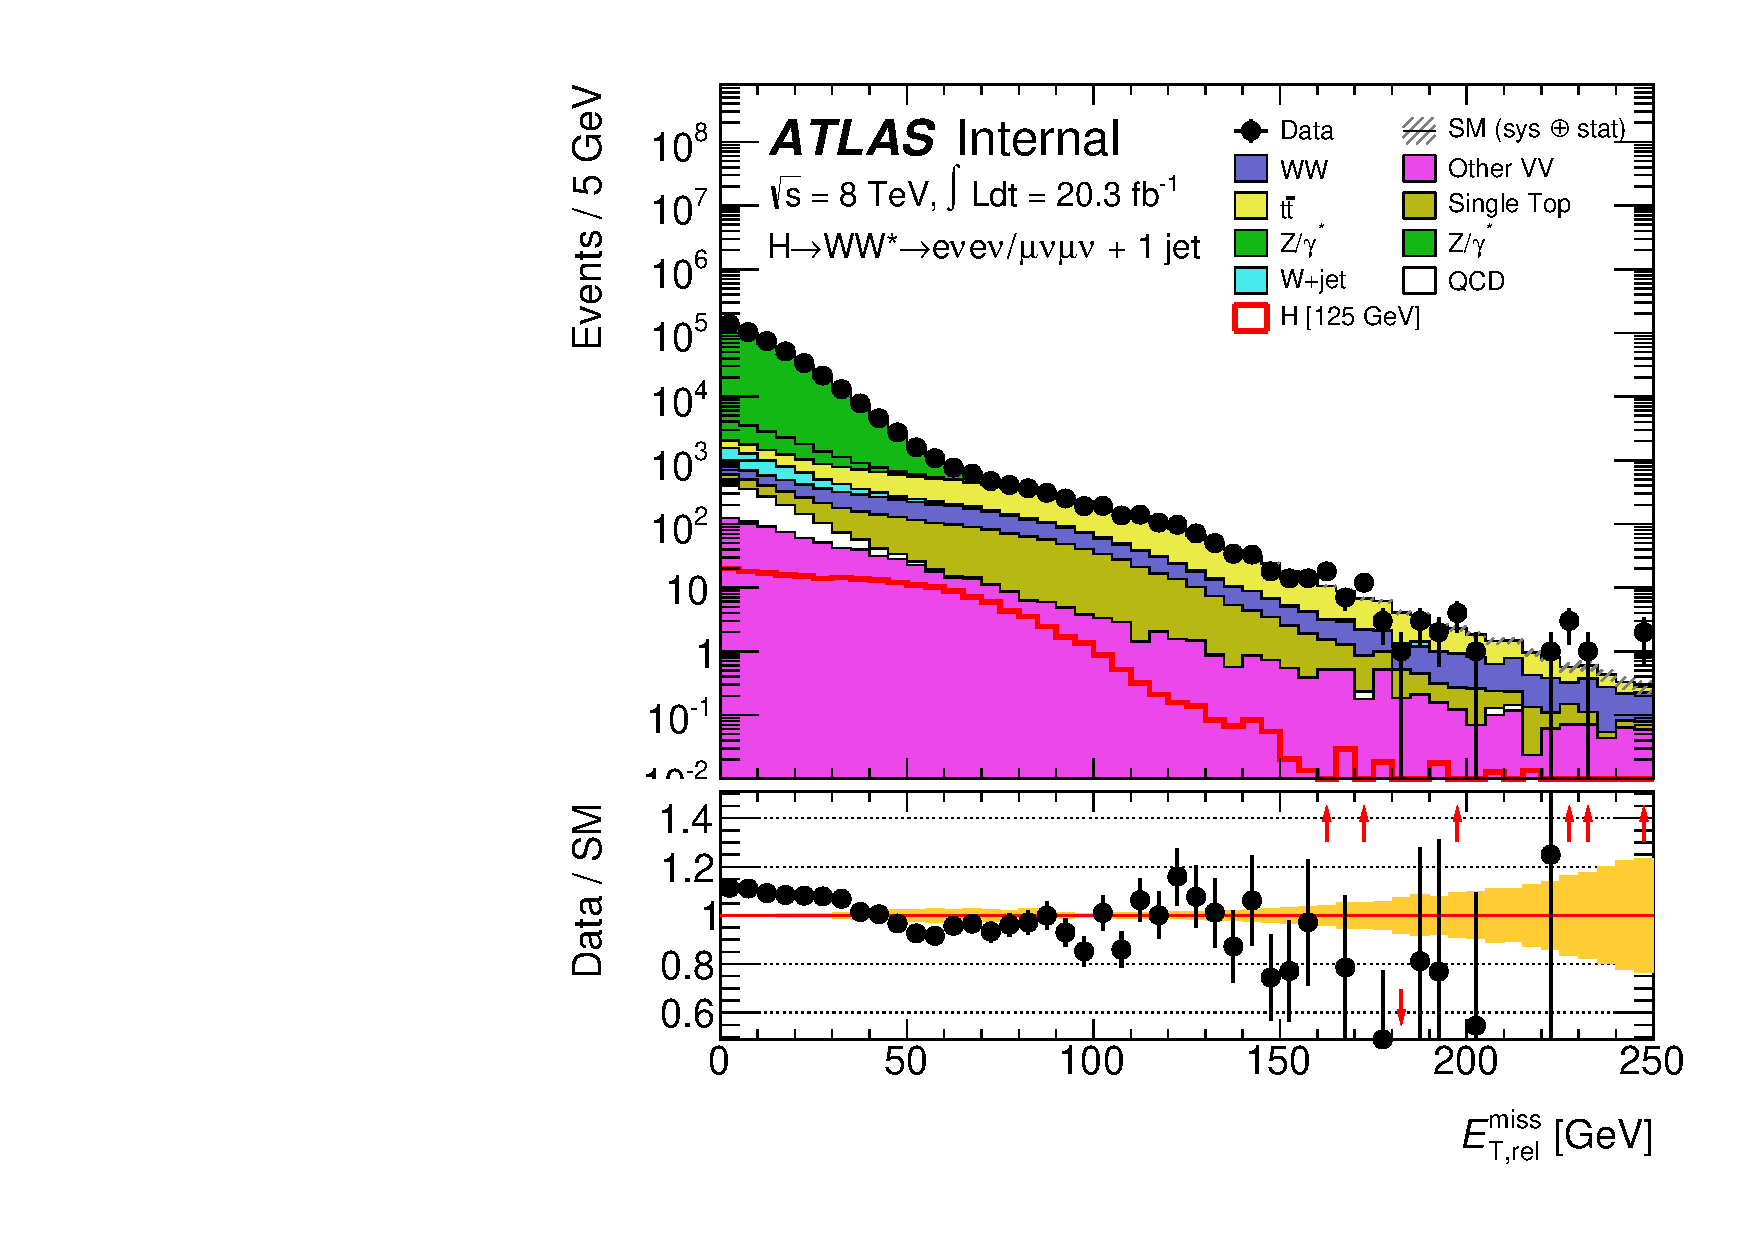
\includegraphics[width=0.495\textwidth]{tex/selection/eemm_CutZVeto_1jet_METRel_mh125_log}
	\\
	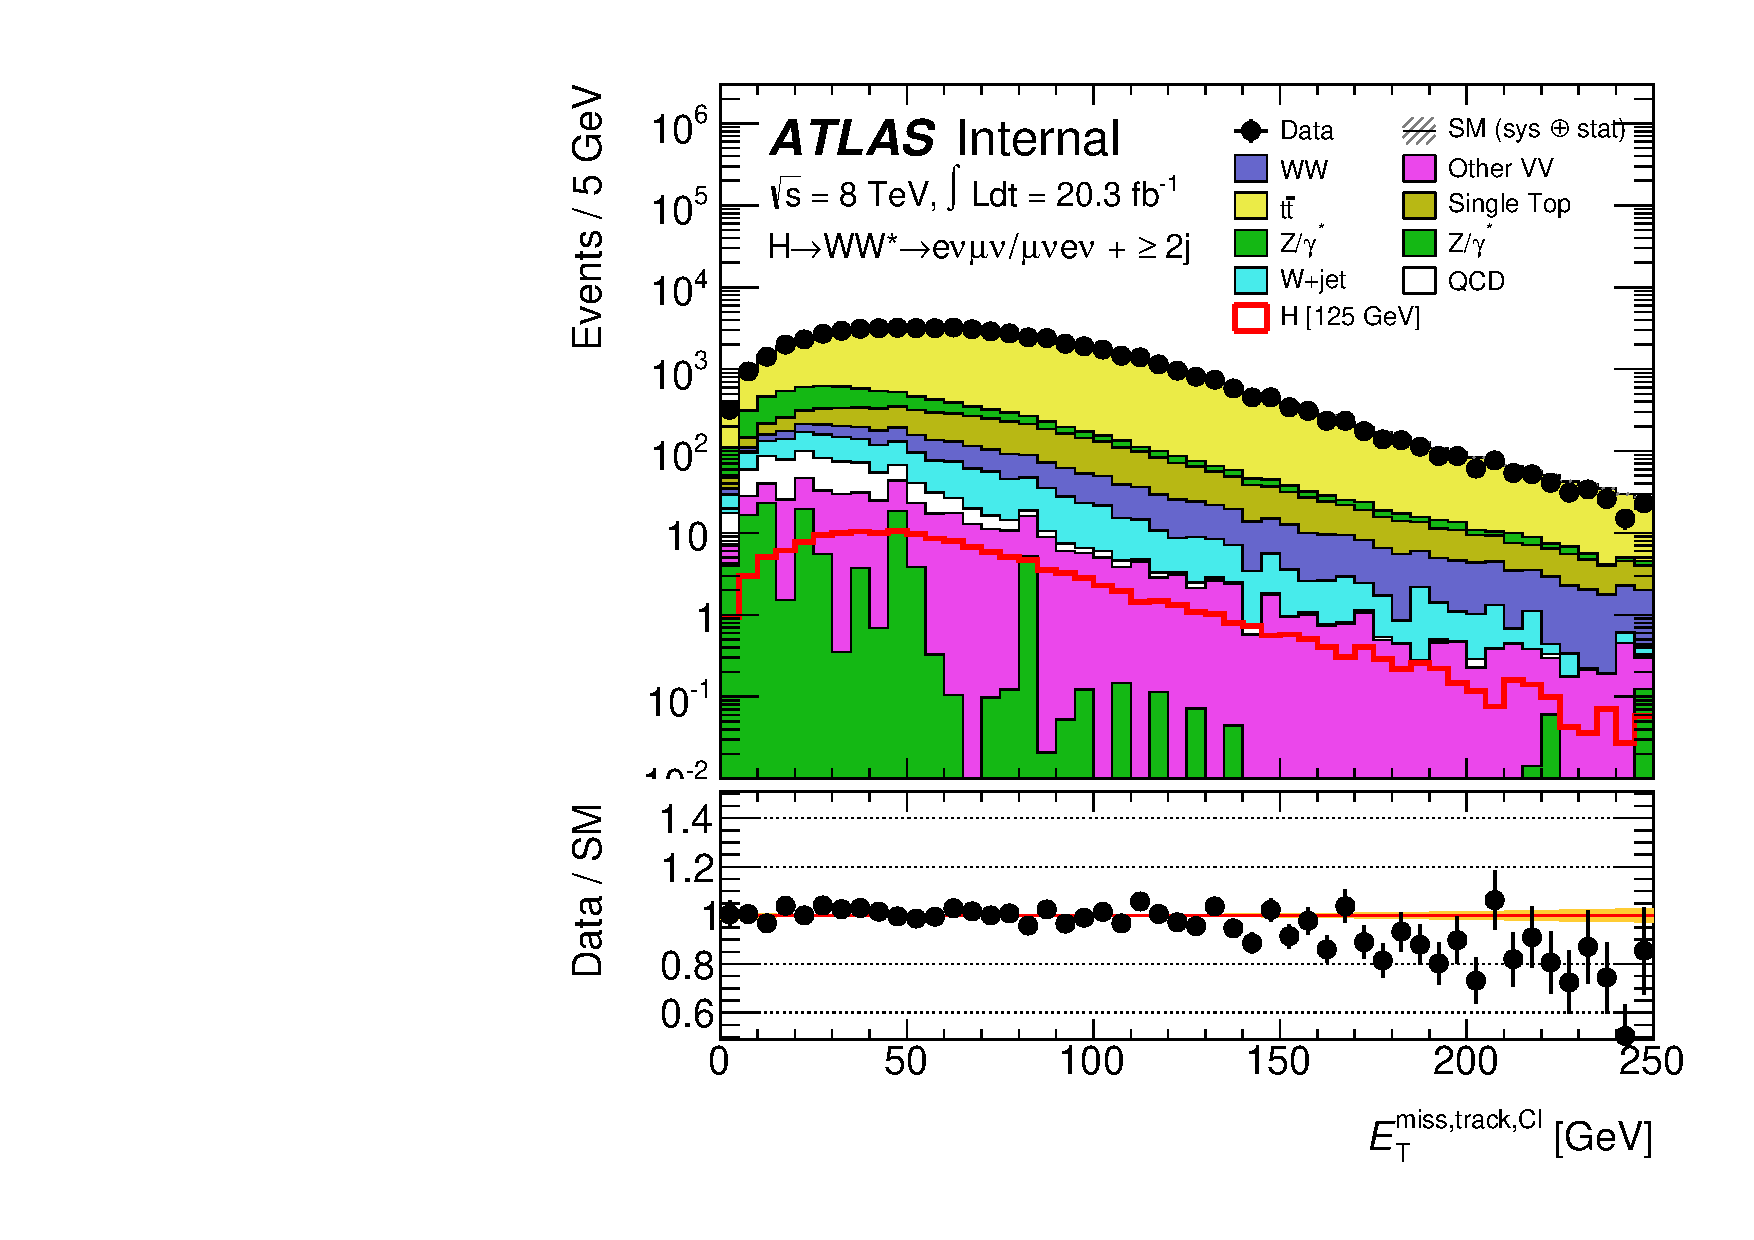
\includegraphics[width=0.495\textwidth]{tex/selection/emme_CutZVeto_2jetincl_MET_TrackHWW_Clj_mh125_log}
	\hfill\null
	\caption{The \met distribution cut upon in the 0-jet (top), 1-jet (middle) and 
	\twojet (bottom) bins, for the \emch/\mech (left) and \eech/\mmch (right) channels.}
	\label{fig:sel:met}
\end{figure}

Requiring significant \met suppresses the \DYll and di-jet backgrounds (see 
\Figure~\ref{fig:sel:met}). Since fake \met is strongly correlated to event kinematics, 
the 0-jet, 1-jet and \twojet bins are considered separately. In the \eech/\mmch channels, 
we require \unit{$\metrel > 40$}{\GeV} in the 0-jet and 1-jet bins (the \eech/\mmch 
channels are not used in the \twojet bin). In the \emch/\mech channels, the \met cut is 
relaxed because the \DYll background is smaller. We require 
\unit{$\corrtrackmet > 20$}{\GeV} in the 0-jet and \twojet bins, and 
\unit{$\corrtrackmet > 10$}{\GeV} in the 1-jet bin.

Following the selection of dilepton events with significant \met, the \emch/\mech 
channels are dominated by top background and the \eech/\mmch channels are dominated by 
\DYll. However, the background composition of all channels is highly dependent upon the 
number of jets (see \Figure~\ref{fig:sel:njets}). Thus, at this stage the analysis is 
binned according to jet multiplicity, so that backgrounds can be targeted individually.

\begin{figure}
	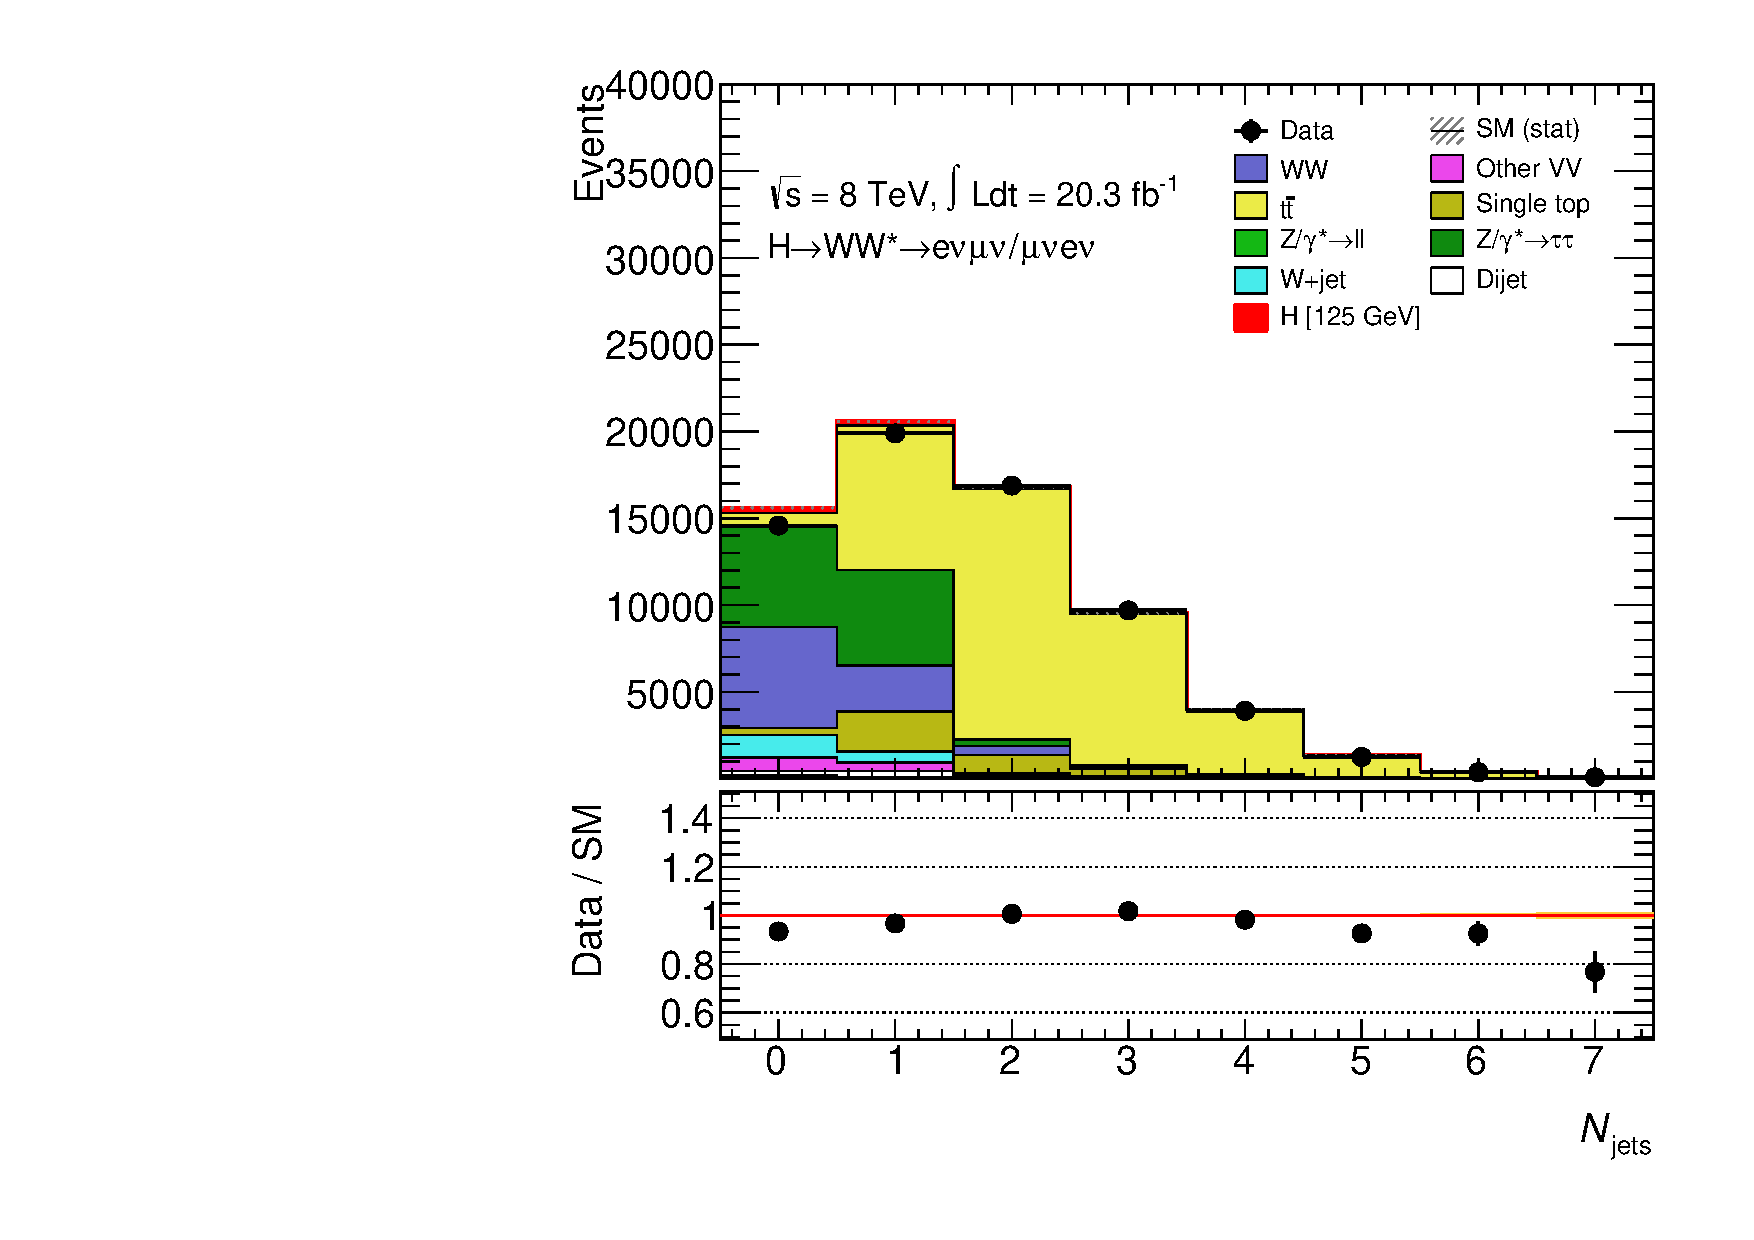
\includegraphics[width=0.495\textwidth]{tex/selection/emme_CutMETRel_m_jet_n_upTo7_mh125_lin}
	\hfill
	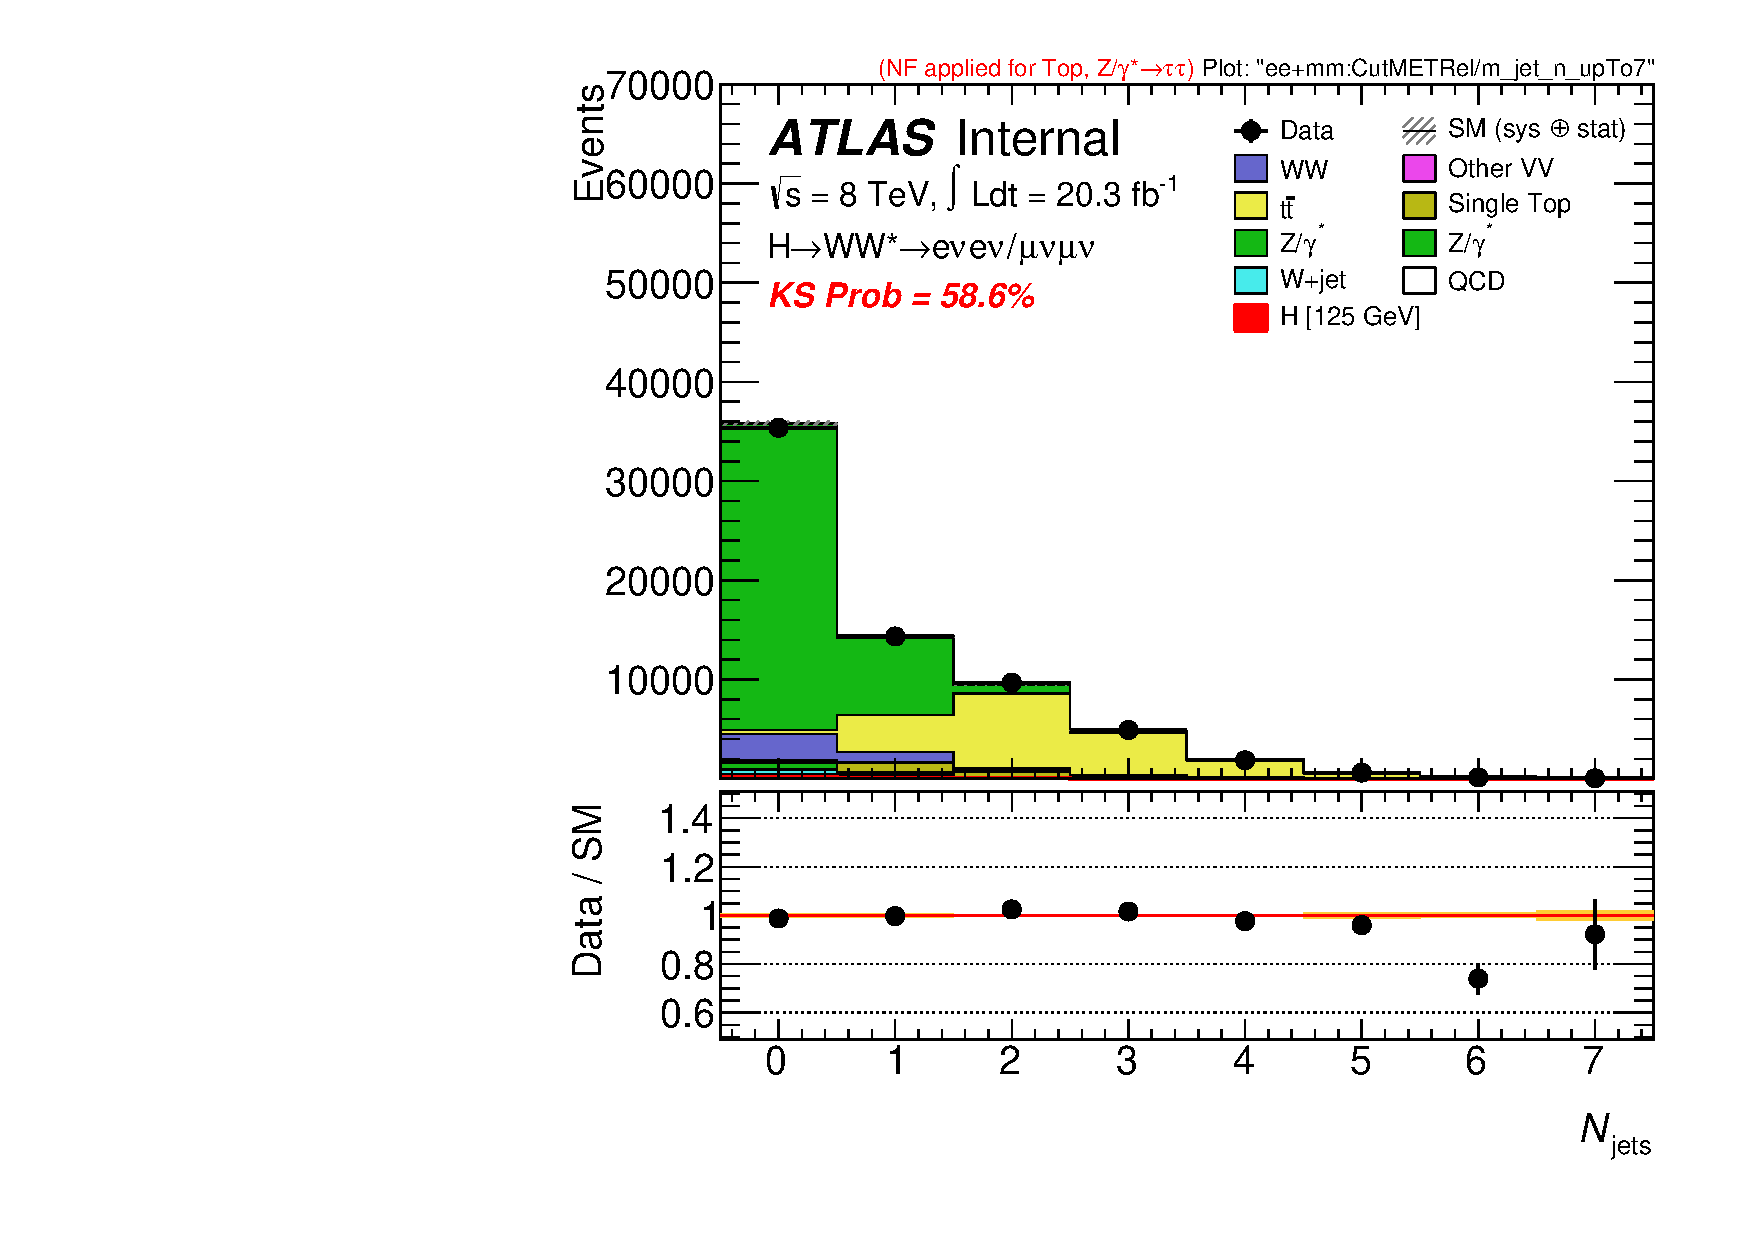
\includegraphics[width=0.495\textwidth]{tex/selection/eemm_CutMETRel_m_jet_n_upTo7_mh125_lin}
	\caption{Jet multiplicity distribution directly preceding jet binning, in the 
	\emch/\mech (left) and \eech/\mmch (right) channels.}
	\label{fig:sel:njets}
\end{figure}



\subsection{\HWWlvlv decay topology}
\label{sec:selection:higgs_decay}

The discrimination of \HWW signal from backgrounds that also feature a \WW pair is a 
problem common to all jet bins. Thus, the topology of the \HWWlvlv decay is discussed 
before continuing with the event selection.

Firstly, the spin-0 nature of the Higgs boson and the \VminusA structure of the weak 
interaction (see \Section~\ref{sec:ewsb}) imply that a small opening angle between the 
two leptons is preferred. This follows from spin conservation and the extremely small 
masses of the neutrinos. Consequently, the mass of the dilepton system, \mll, is also 
small. This follows from $m_{\Plepton\Plepton}^2 \simeq m_{\Plepton_1}^2 + 
m_{\Plepton_2}^2 + 2 E_{\Plepton_1} E_{\Plepton_2} \parenths{1 - \cos\vartheta}$, where 
$\vartheta$ is the opening angle. Thus, signal events are selected with the criteria 
$\dphill < 1.8$ and \unit{$\mll < 55$}{\GeV}.

Secondly, the invariant mass of the dilepton and dineutrino system should correspond to 
\mH (modified by a Breit-Wigner distribution). Unfortunately, as discussed above, it is 
only possible to infer the \textit{transverse} component of the dineutrino system 
momentum. We therefore construct a transverse mass variable
\begin{equation}
	\mt = \sqrt{\parenths{\etll + \corrtrackmet}^2 - \mods{\ptllvec + \corrtrackmetvec}^2}
\end{equation}
where $E_{\text{T,\HepProcess{\Plepton\Plepton}}}^2 = 
p_{\text{T,\HepProcess{\Plepton\Plepton}}}^2 + m_{\Plepton\Plepton}^2$ and 
\corrtrackmetvec 
is used as it has the best resolution (see \Section~\ref{sec:objects:met}). At 
hadron-level this is an event-by-event lower bound on \mH, though at detector-level the 
sharp cut-off is smeared by the poor \corrtrackmet resolution. \mt is used in the 
statistical fitting procedure.



\subsection{0-jet selection}
\label{sec:selection:0j}

The 0-jet bin is dominated by \DY and \WW backgrounds. A small number of pathological 
events where \metvec is near \ptllvec are rejected by requiring $\dphillmet > \pi/2$.

Considering the \DYll background, the boson \pt will generally be less than the \pt 
threshold used in jet selection, since no jet has been found. Thus, the \DY background is 
greatly reduced by requiring \unit{$\ptll > 30$}{\GeV} (see 
\Figure~\ref{fig:sel:0j:ptll}). In the \eech/\mmch channels only, the \DYll background is 
also suppressed by an additional cut \unit{$\corrtrackmet > 40$}{\GeV} (see 
\Figure~\ref{fig:sel:0j:sf_cuts}).

\begin{figure}
	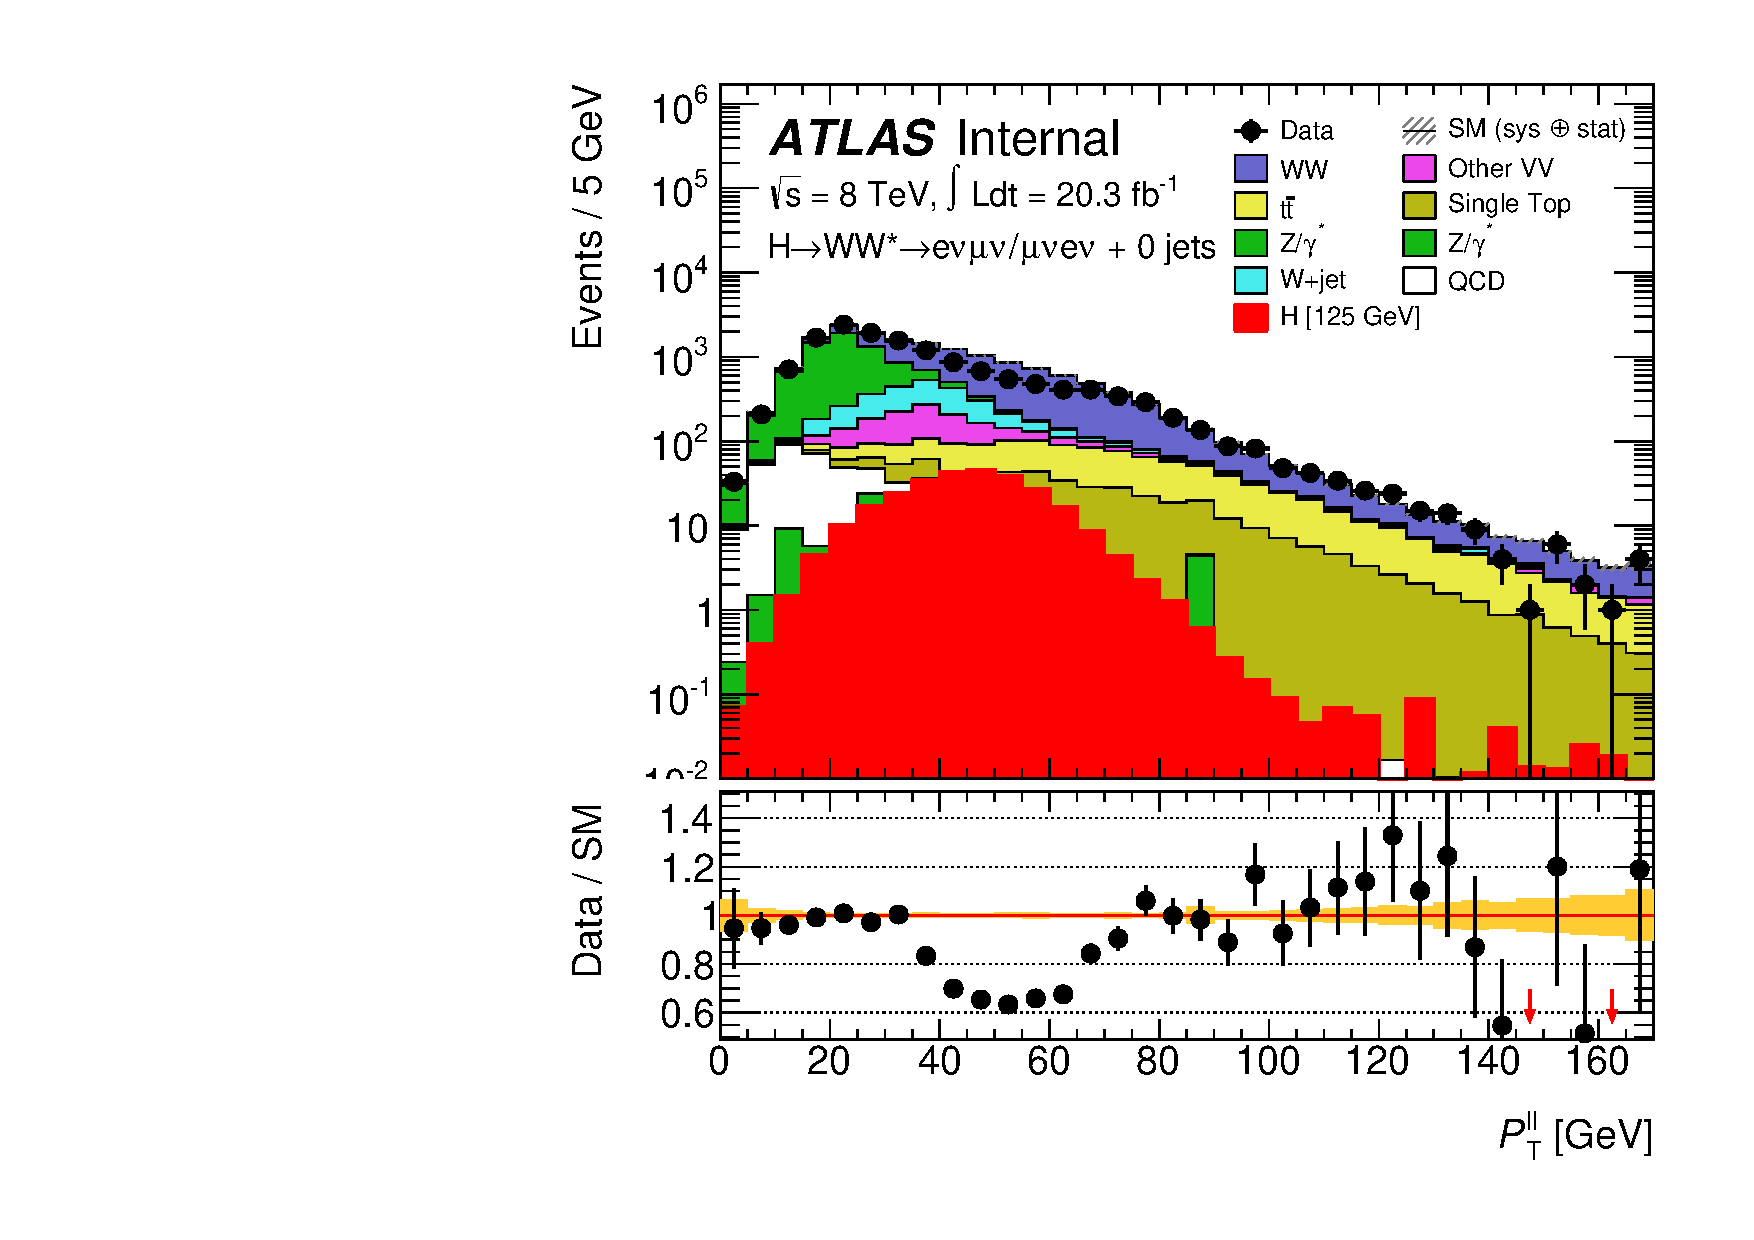
\includegraphics[width=0.495\textwidth]{tex/selection/emme_CutDPhillMET_0jet_Ptll_mh125_log}
	\hfill
	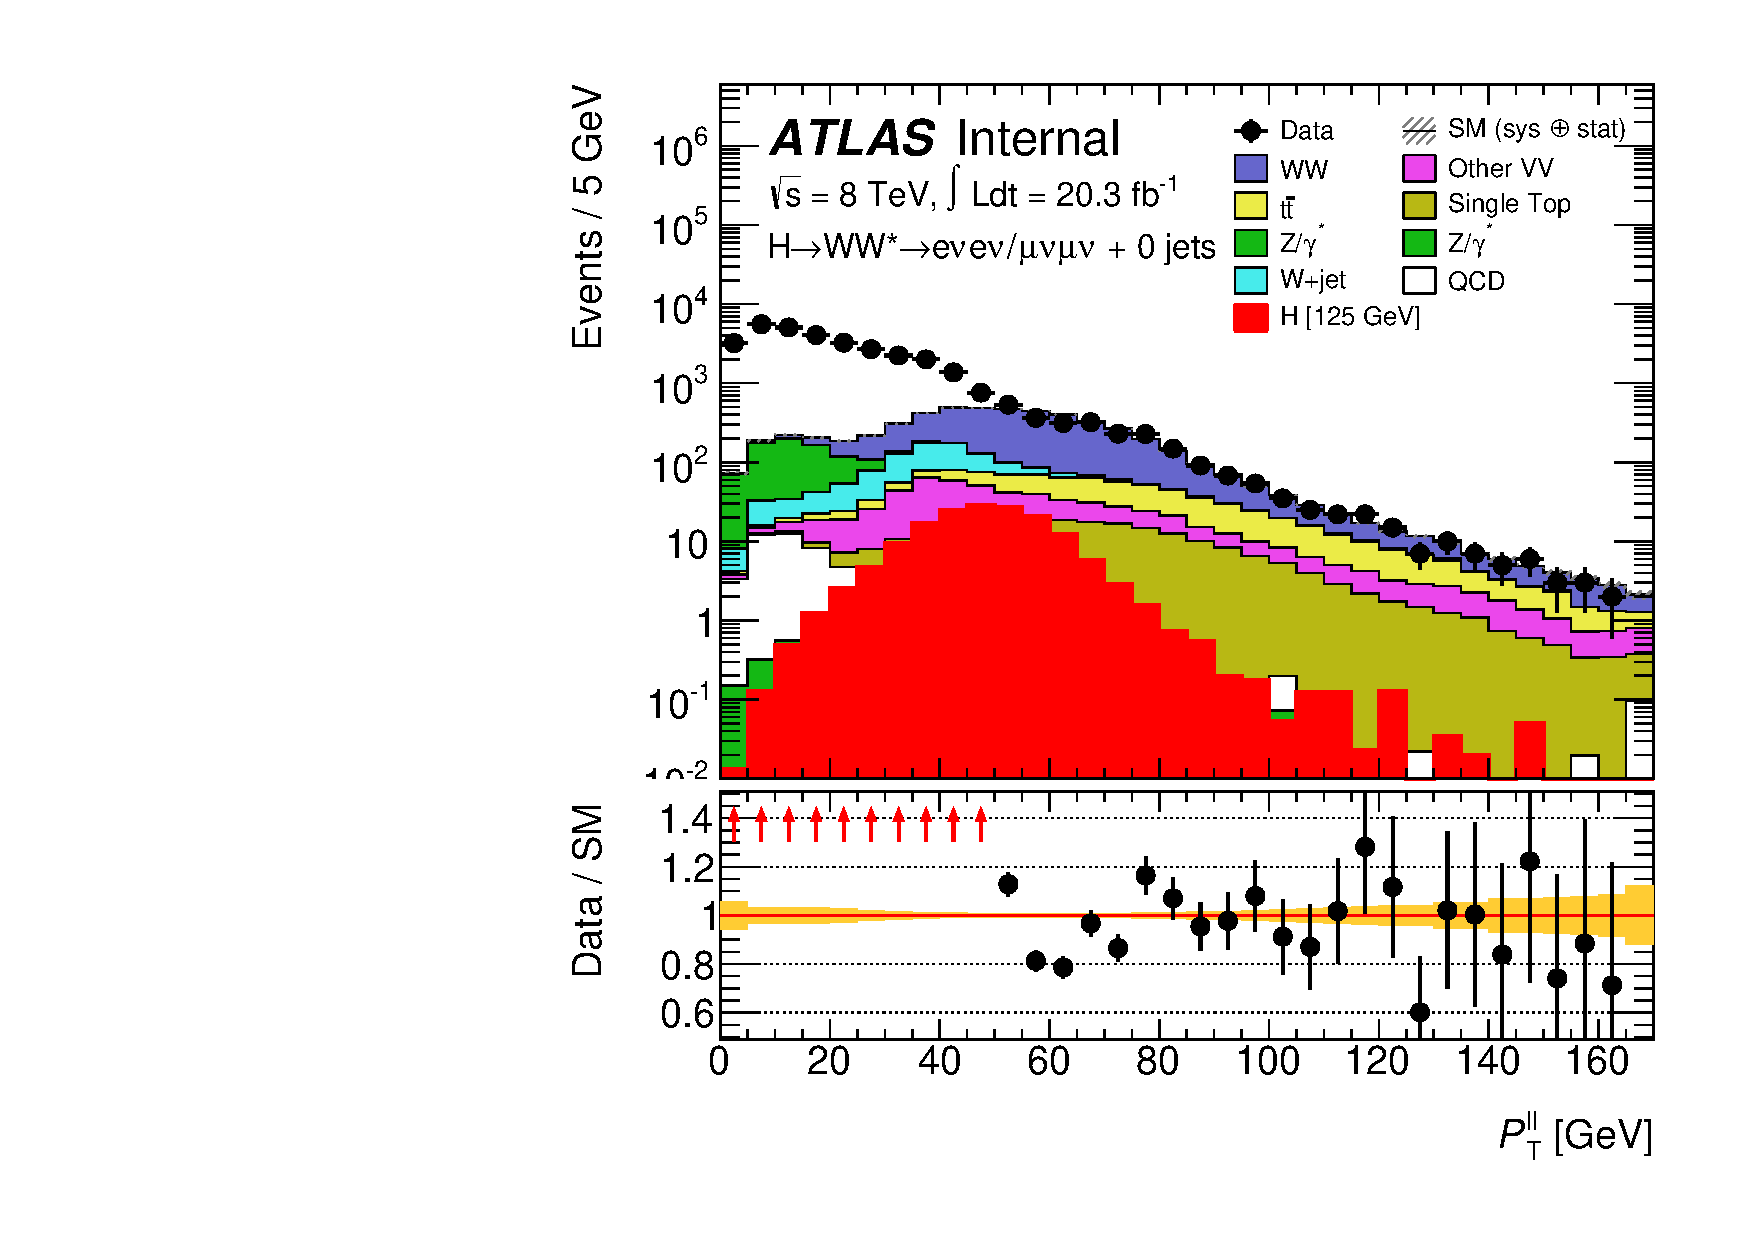
\includegraphics[width=0.495\textwidth]{tex/selection/eemm_CutDPhillMET_0jet_Ptll_mh125_log}
	\caption{The \ptll distribution directly before it is cut upon, in the \emch/\mech (left) 
	and \eech/\mmch (right) channels.}
	\label{fig:sel:0j:ptll}
\end{figure}

After the signal topology selection (see \Section~\ref{sec:selection:higgs_decay}), a 
large \DYll background remains in the \eech/\mmch channels, despite the significant \met 
requirements. This can be further suppressed by searching for soft hadronic activity to 
balance the dilepton system. First, jets with \unit{$\pt > 10$}{\GeV} and $\mods{\eta} < 
4.5$ are found (as detailed in \Section~\ref{sec:objects:jets}, minus the JVF cut). 
Then a discriminant is defined
\begin{equation}
	\frecoil = \left. \mods{\sum\limits_{j\text{ in }\wedge} \text{JVF}_{j} \cdot \bvec{p}_{\text{T,}j}} \, \middle/ \ptll \right.
	\label{eq:frecoil}
\end{equation}
where $\wedge$ is the detector quadrant centred on $-\ptllvec$. This is essentially the 
fraction of \ptll that can be balanced by soft hadronic activity in the opposing quadrant,
and so is larger in \DYll than processes with neutrinos. We require $\frecoil < 0.1$ in 
the \eech/\mmch channels (see \Figure~\ref{fig:sel:0j:sf_cuts}). \frecoil is also 
instrumental in estimating the \DYll background, and shall be revisited in 
\Section~\ref{sec:dy}.

\begin{figure}
	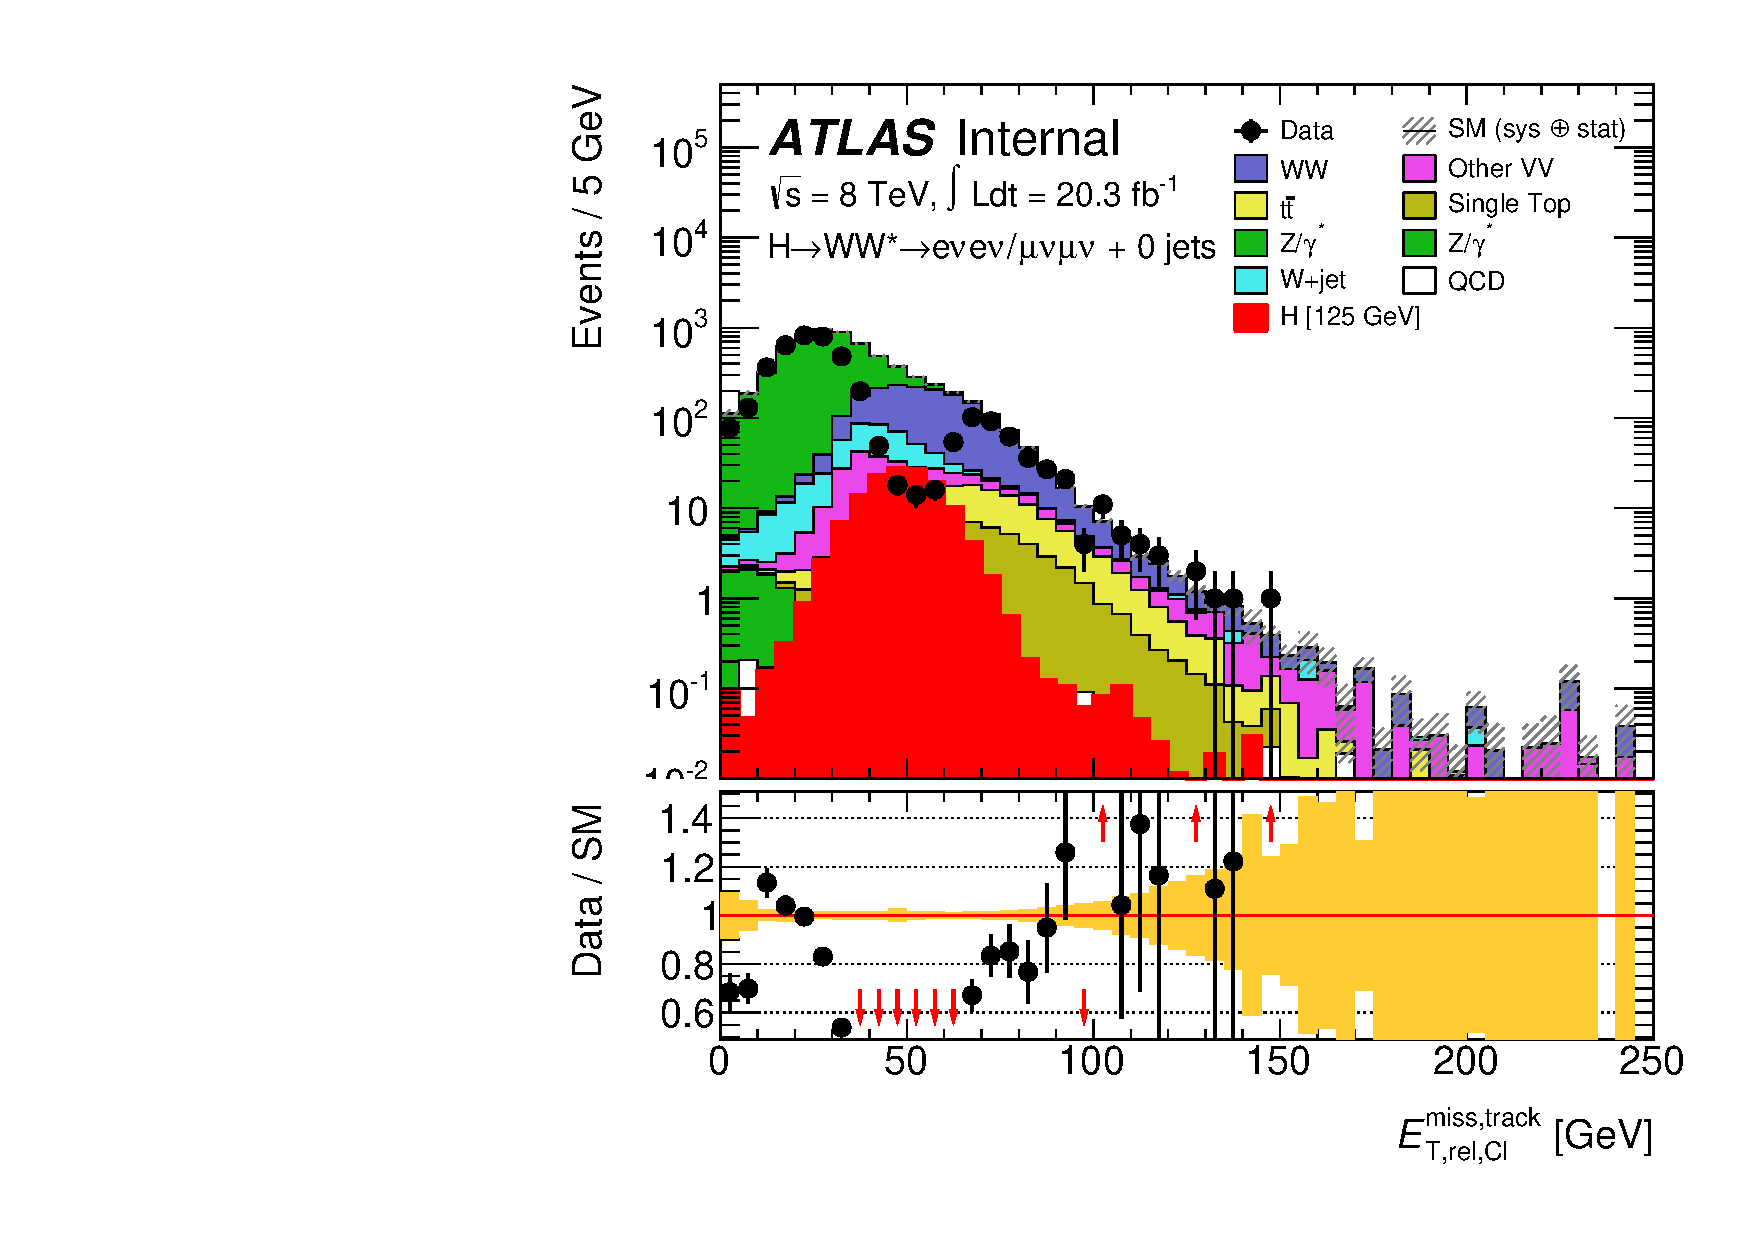
\includegraphics[width=0.495\textwidth]{tex/selection/eemm_CutTopoMll_0jet_METRel_TrackHWW_Clj_mh125_log}
	\hfill
	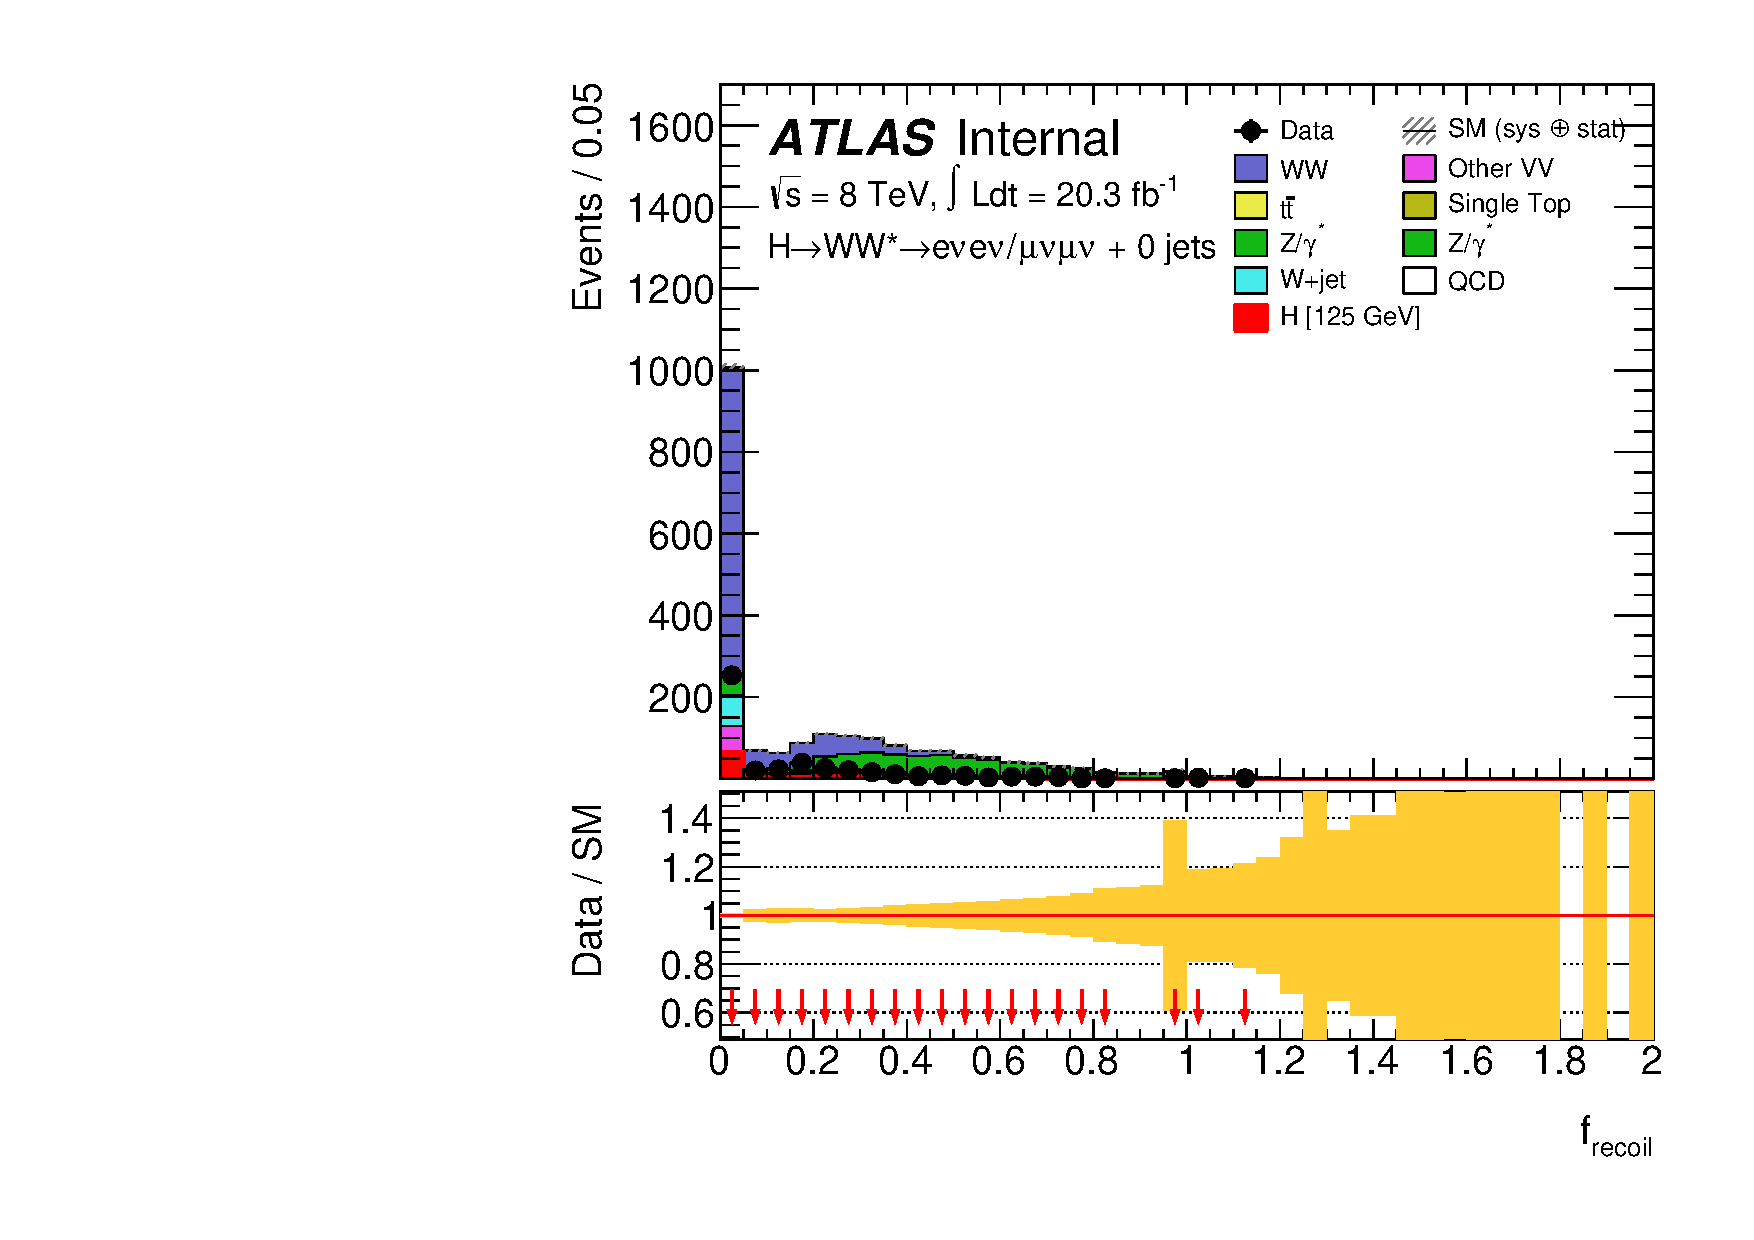
\includegraphics[width=0.495\textwidth]{tex/selection/eemm_CutTopoDPhill_0jet_f_recoil_mh125_lin}
	\caption{The \corrtrackmetrel (left) and \frecoil (right) distributions directly 
	before they are cut upon in the \eech/\mmch channels.}
	\label{fig:sel:0j:sf_cuts}
\end{figure}

The event yields of the 0-jet selection are provided in \Appendix~\ref{app:sr_yields}, 
and the \mt distributions of the selected events are shown in \Figure~\ref{fig:sel:0j:mt}.

\begin{figure}
	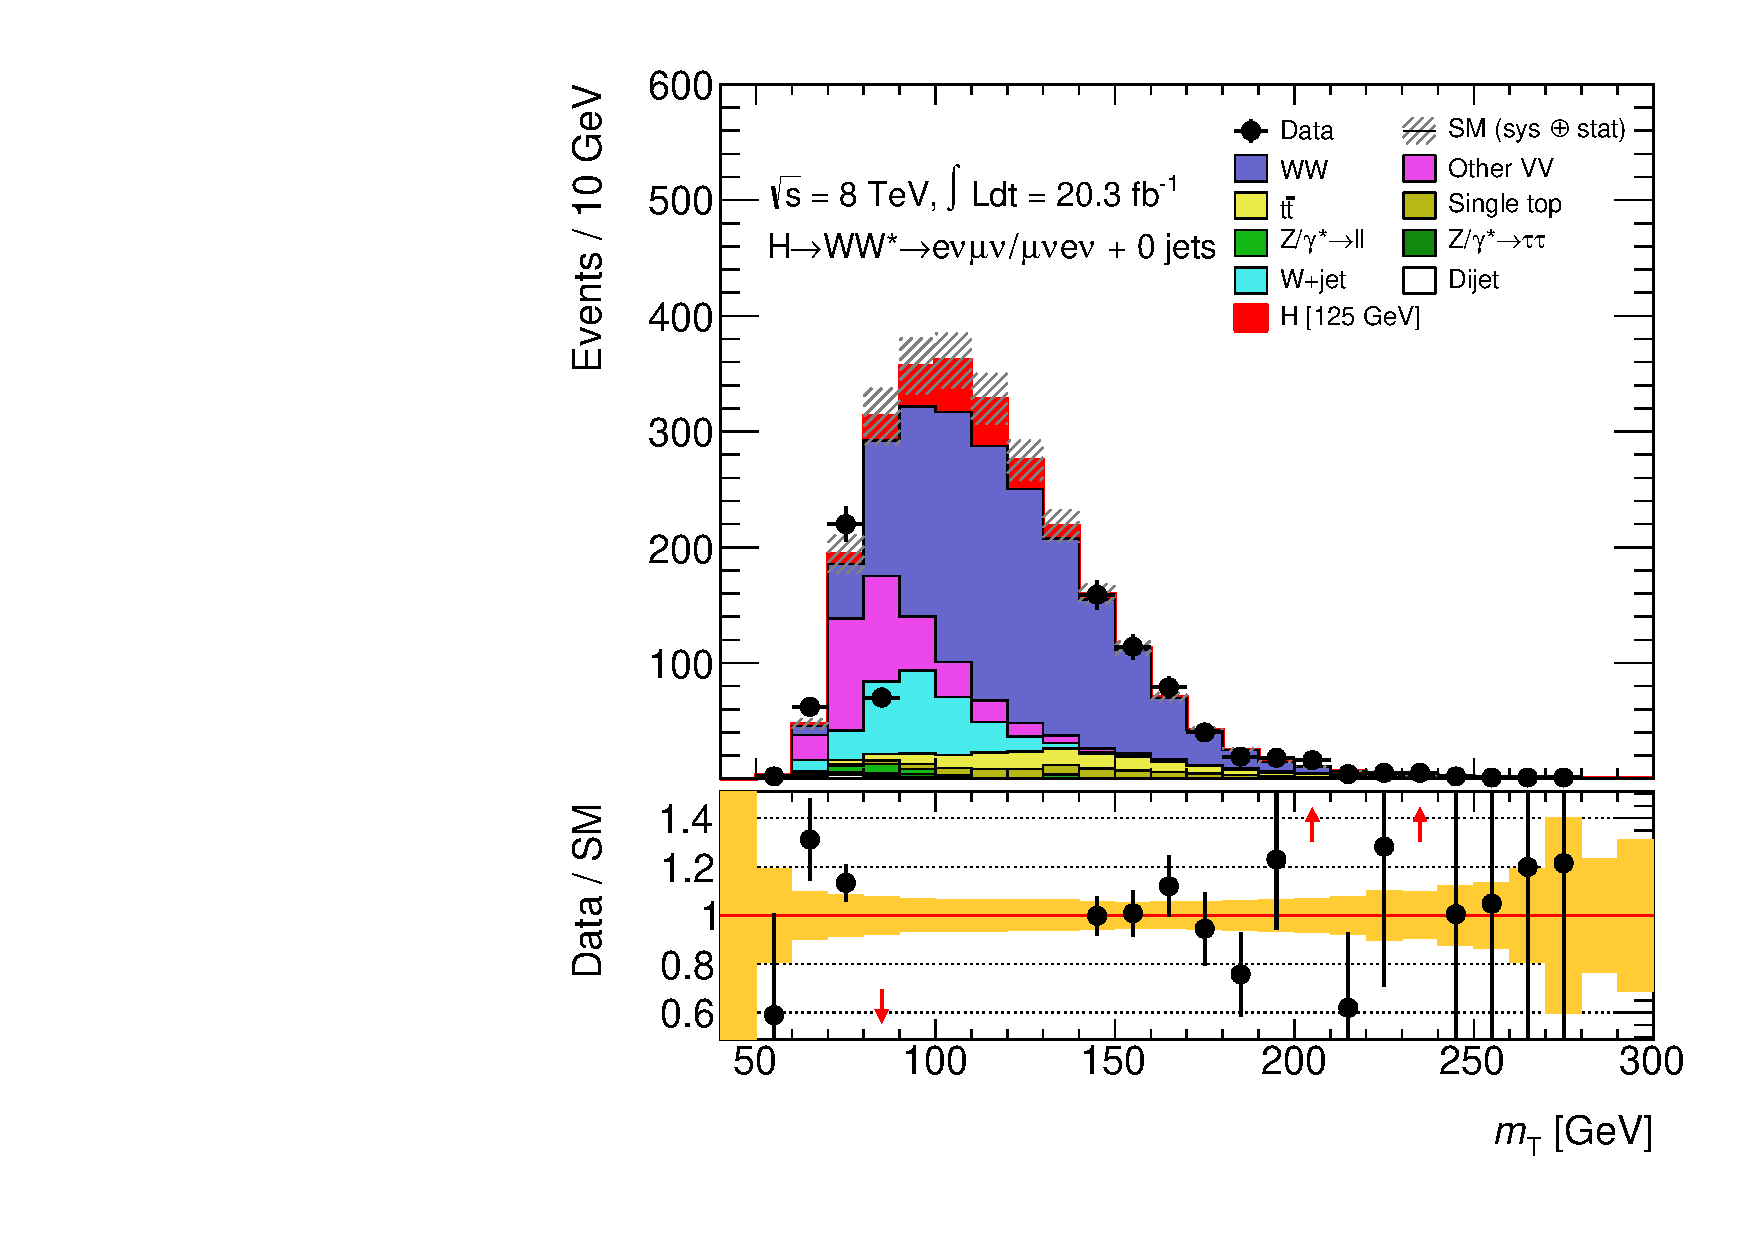
\includegraphics[width=0.495\textwidth]{tex/selection/emme_CutFRecoil_0jet_MT_TrackHWW_Clj_mh125_lin}
	\hfill
	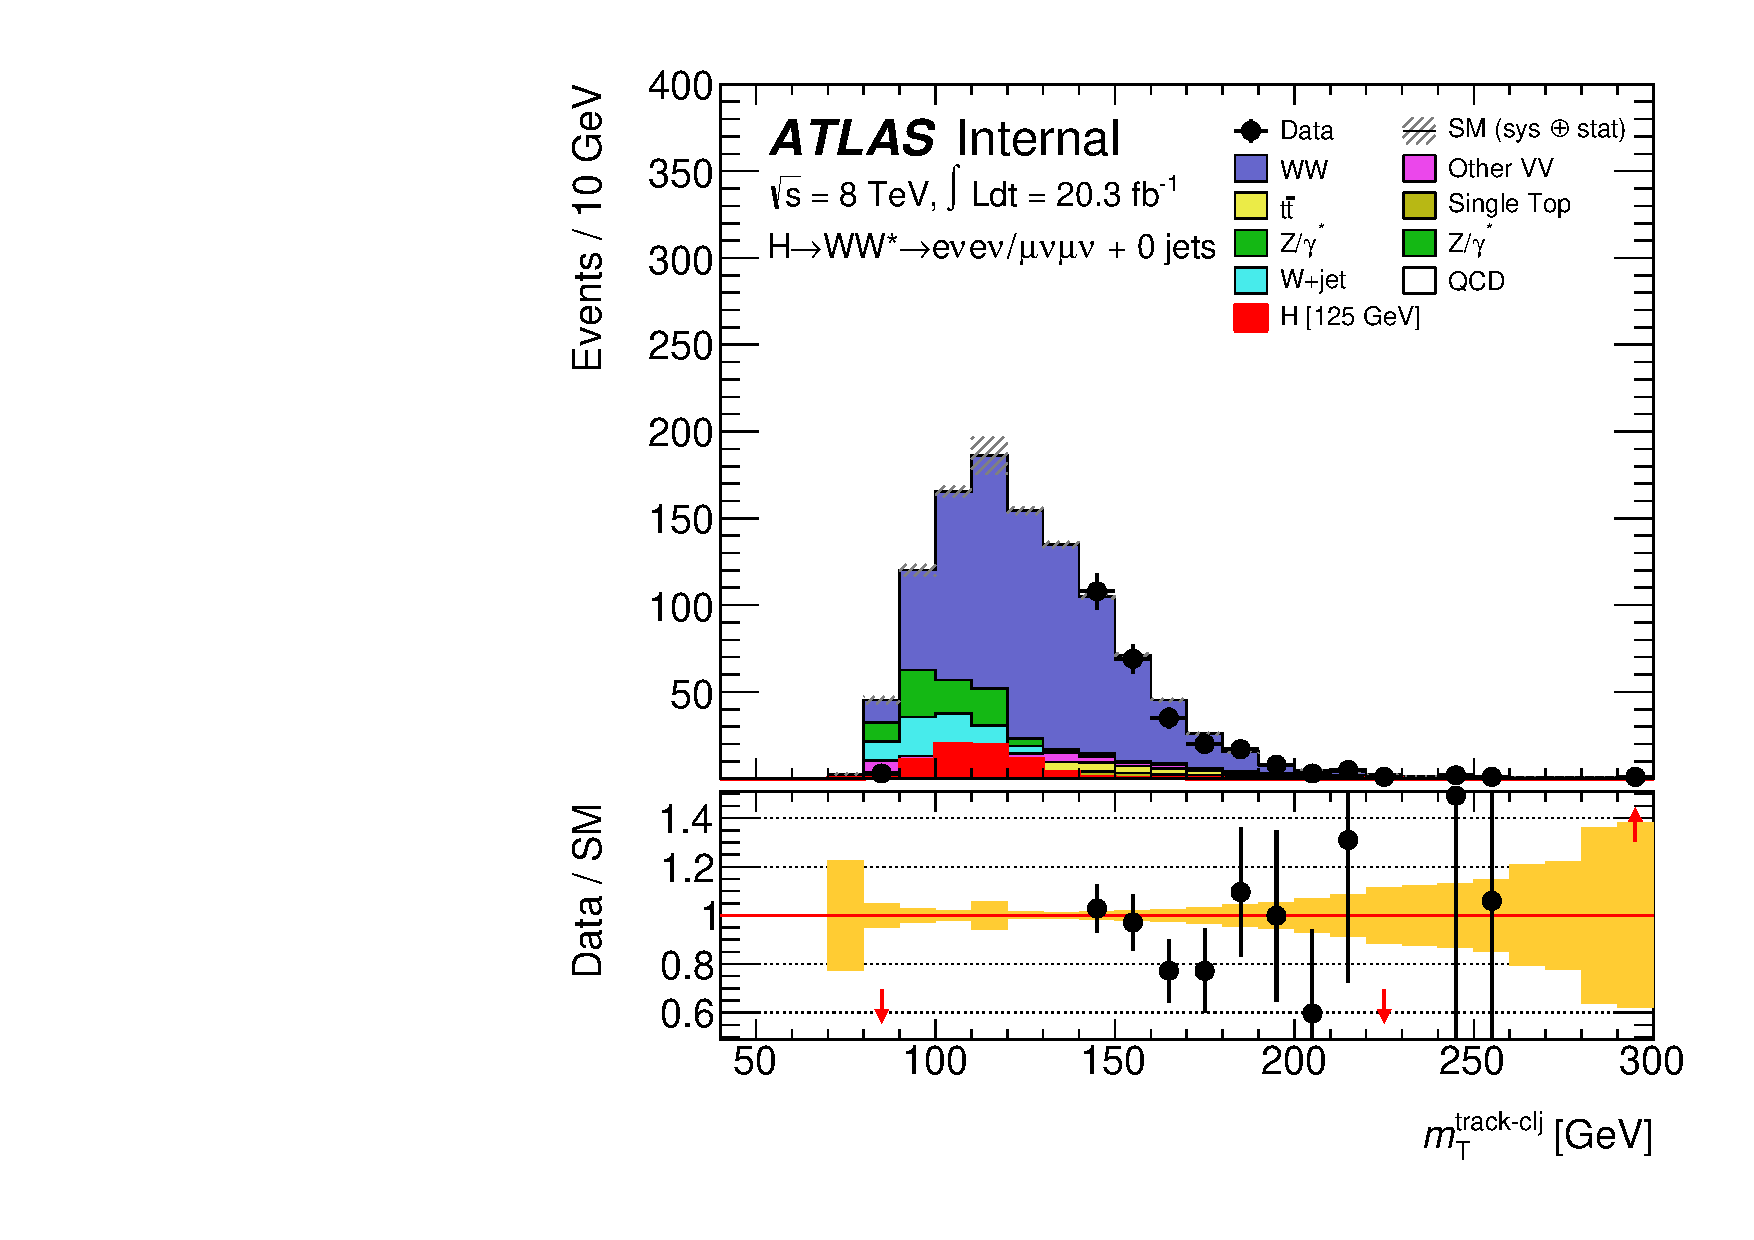
\includegraphics[width=0.495\textwidth]{tex/selection/eemm_CutFRecoil_0jet_MT_TrackHWW_Clj_mh125_lin}
	\caption{The \mt distribution of the selected 0-jet events, in the \emch/\mech (left) and 
	\eech/\mmch (right) channels.}
	\label{fig:sel:0j:mt}
\end{figure}



\subsection{1-jet selection}
\label{sec:selection:1j}

The 1-jet bin is initially dominated by the \DY and top backgrounds (see 
\Figure~\ref{fig:sel:njets}), though the top background is efficiently reduced by vetoing 
events containing a \Pbottom-tagged jet with \unit{$\pt > 20$}{\GeV} (see 
\Section~\ref{sec:objects:bjets}).

The \emch/\mech pre-selection has a loose \corrtrackmet cut in order to maximise the 
signal acceptance. However, this yields a sizeable di-jet background, which has a large 
uncertainty. For this reason, two single-lepton transverse mass variables are constructed
\begin{equation}
	m_{\text{T,}\Plepton_i} = \sqrt{2 \, p_{\text{T,}\Plepton_i} \, \corrtrackmet 
	\sqbracs{1 - \cos\Delta\phi\parenths{\Plepton_i, \corrtrackmet}}} \,.
\end{equation}
Their maximum, \maxmtw, tends to peak at lower values for processes with fake \met (see 
\Figure~\ref{fig:sel:1j:df_cuts}). Therefore we require \unit{$\maxmtw > 50$}{\GeV}.

\begin{figure}
	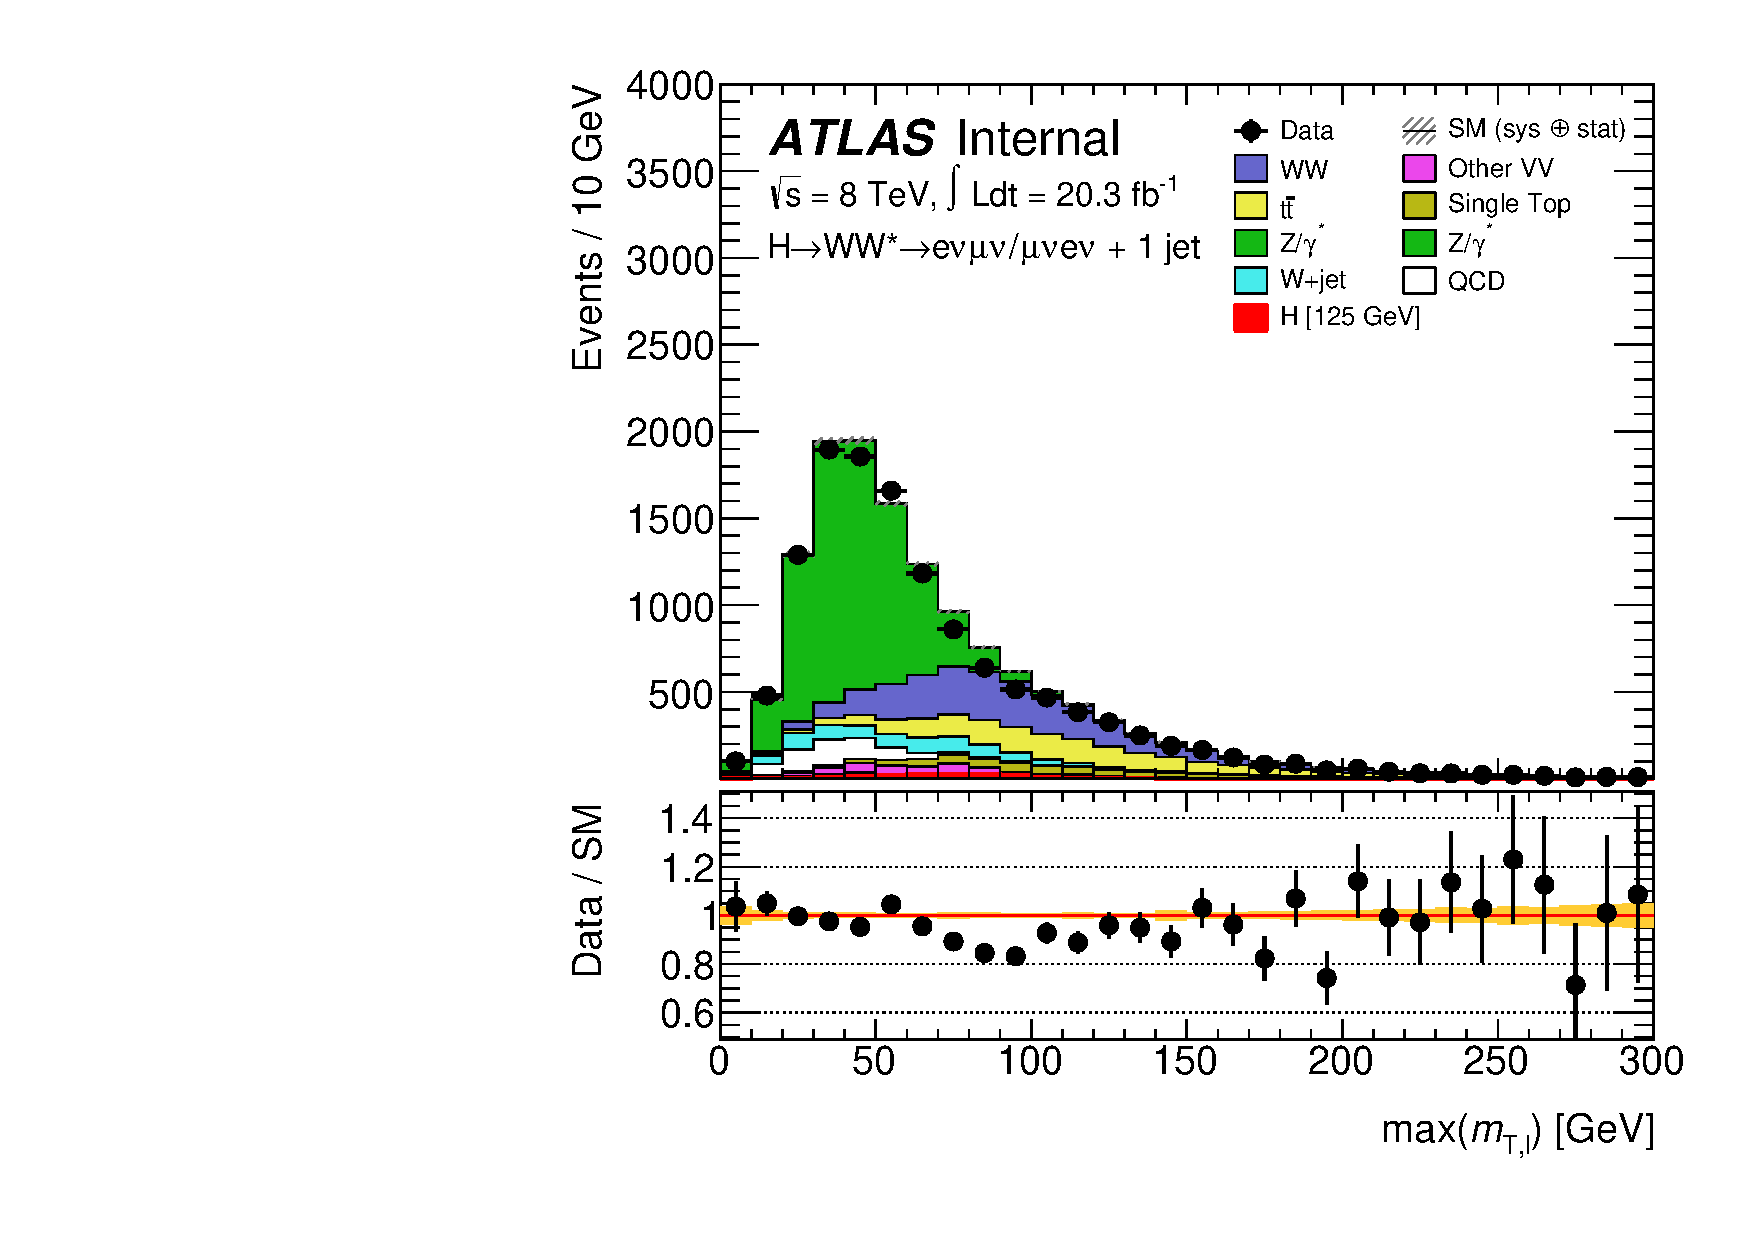
\includegraphics[width=0.495\textwidth]{tex/selection/emme_CutbVeto_1jet_MaxMTW_TrackHWW_Clj_mh125_lin}
	\hfill
	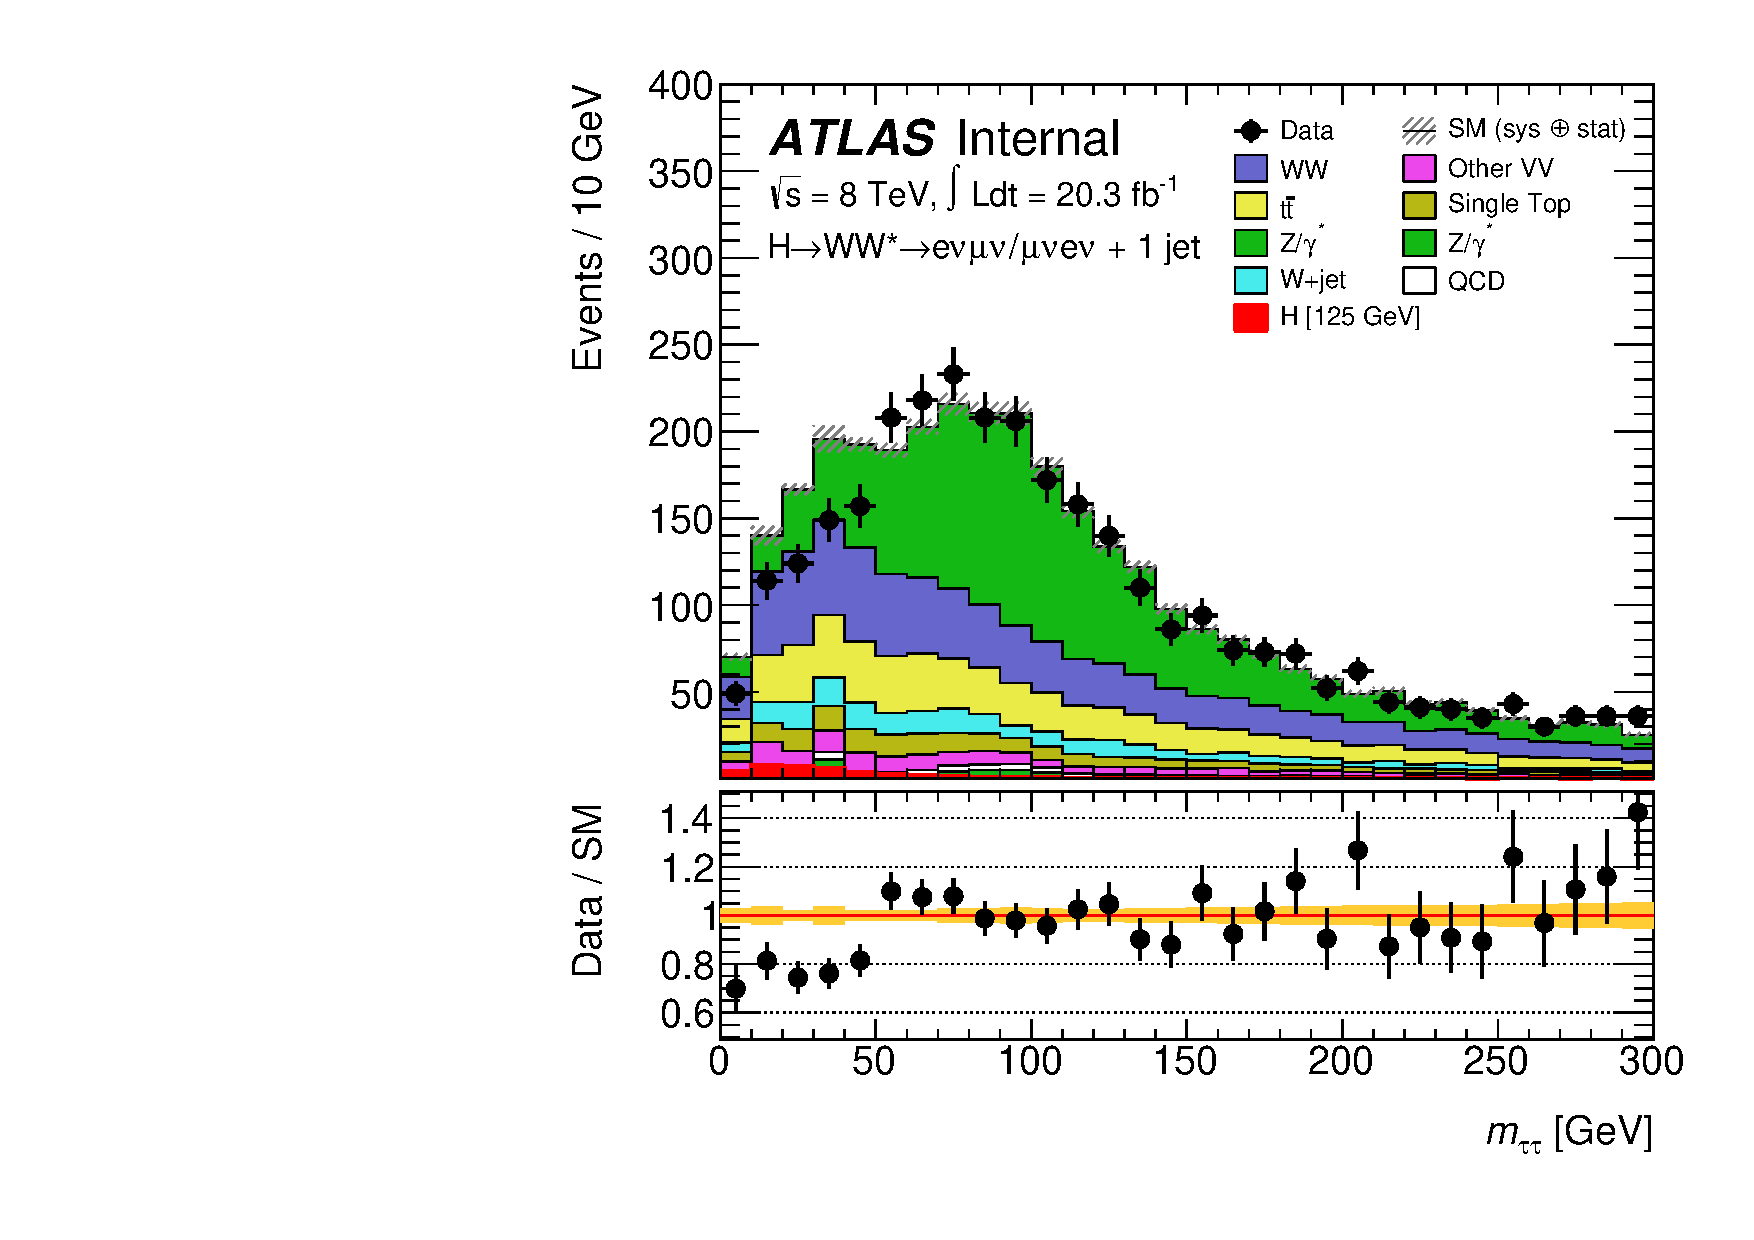
\includegraphics[width=0.495\textwidth]{tex/selection/emme_CutMaxMTlep_1jet_Mtt_TrackHWW_Clj_mh125_lin}
	\caption{The \maxmtw (left) and \mtautau (right) distributions directly 
	before they are cut upon in the \emch/\mech channels.}
	\label{fig:sel:1j:df_cuts}
\end{figure}

At this stage, the \DYtt background dominates the \emch/\mech channels. To aid 
discrimination, a di-tau mass is constructed
\begin{equation}
	\mtautau = 
		\begin{cases}
			\mll \,/ \sqrt{x_1 x_2} &\text{if}~x_1, x_2 > 0 \\
			0 &\text{otherwise}
		\end{cases}
\end{equation}
where $x_i$ is the \pt fraction of the $i$th \Ptau imparted to the $i$th lepton. As $x_i$ 
cannot be directly measured using individual neutrino momenta, \corrtrackmet is split by 
assuming the \Ptau decays collinearly, \ie 
$\Delta\phi\parenths{\Plepton,\HepProcess{\Pnut\Pnulepton}} = 0$. 
This approximation is reasonable since each \Ptau has large \pt. We require 
\unit{$\mtautau < \mZ - 25$}{\GeV} (see \Figure~\ref{fig:sel:1j:df_cuts}).

After the signal topology selection, the \DYll background is suppressed in the 
\eech/\mmch channels by requiring \unit{$\trackmetrel > 35$}{\GeV} and $\frecoil < 0.1$ 
(see \Figure~\ref{fig:sel:1j:sf_cuts}). In the 1-jet bin, the \frecoil definition is 
altered with respect to (\ref{eq:frecoil}): the quadrant $\wedge$ is centred upon 
$-\ptlljvec$ and the denominator becomes \ptllj. This is because a hard jet has been 
found, and so it is the dilepton + jet system that must be balanced by the hard recoil.

\begin{figure}
	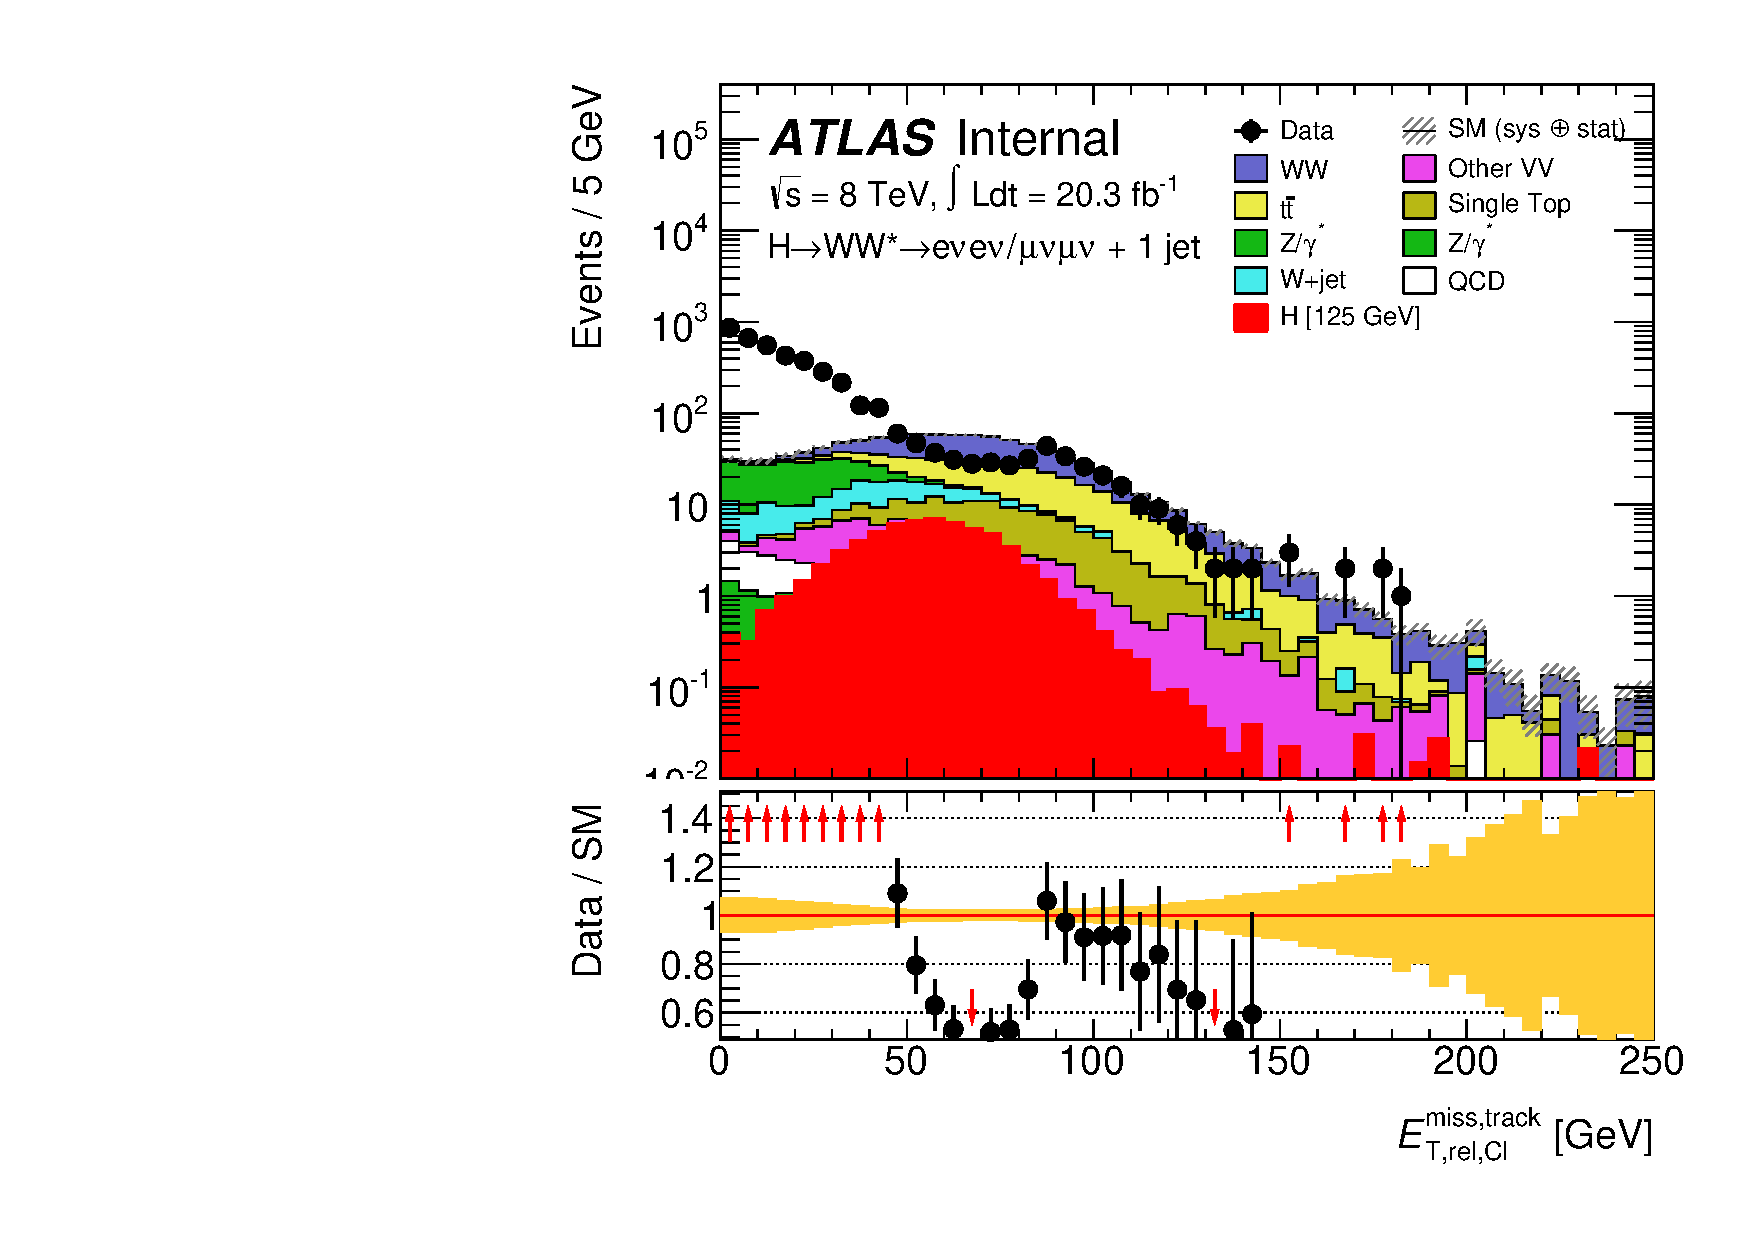
\includegraphics[width=0.495\textwidth]{tex/selection/eemm_CutTopoMll_1jet_METRel_TrackHWW_Clj_mh125_log}
	\hfill
	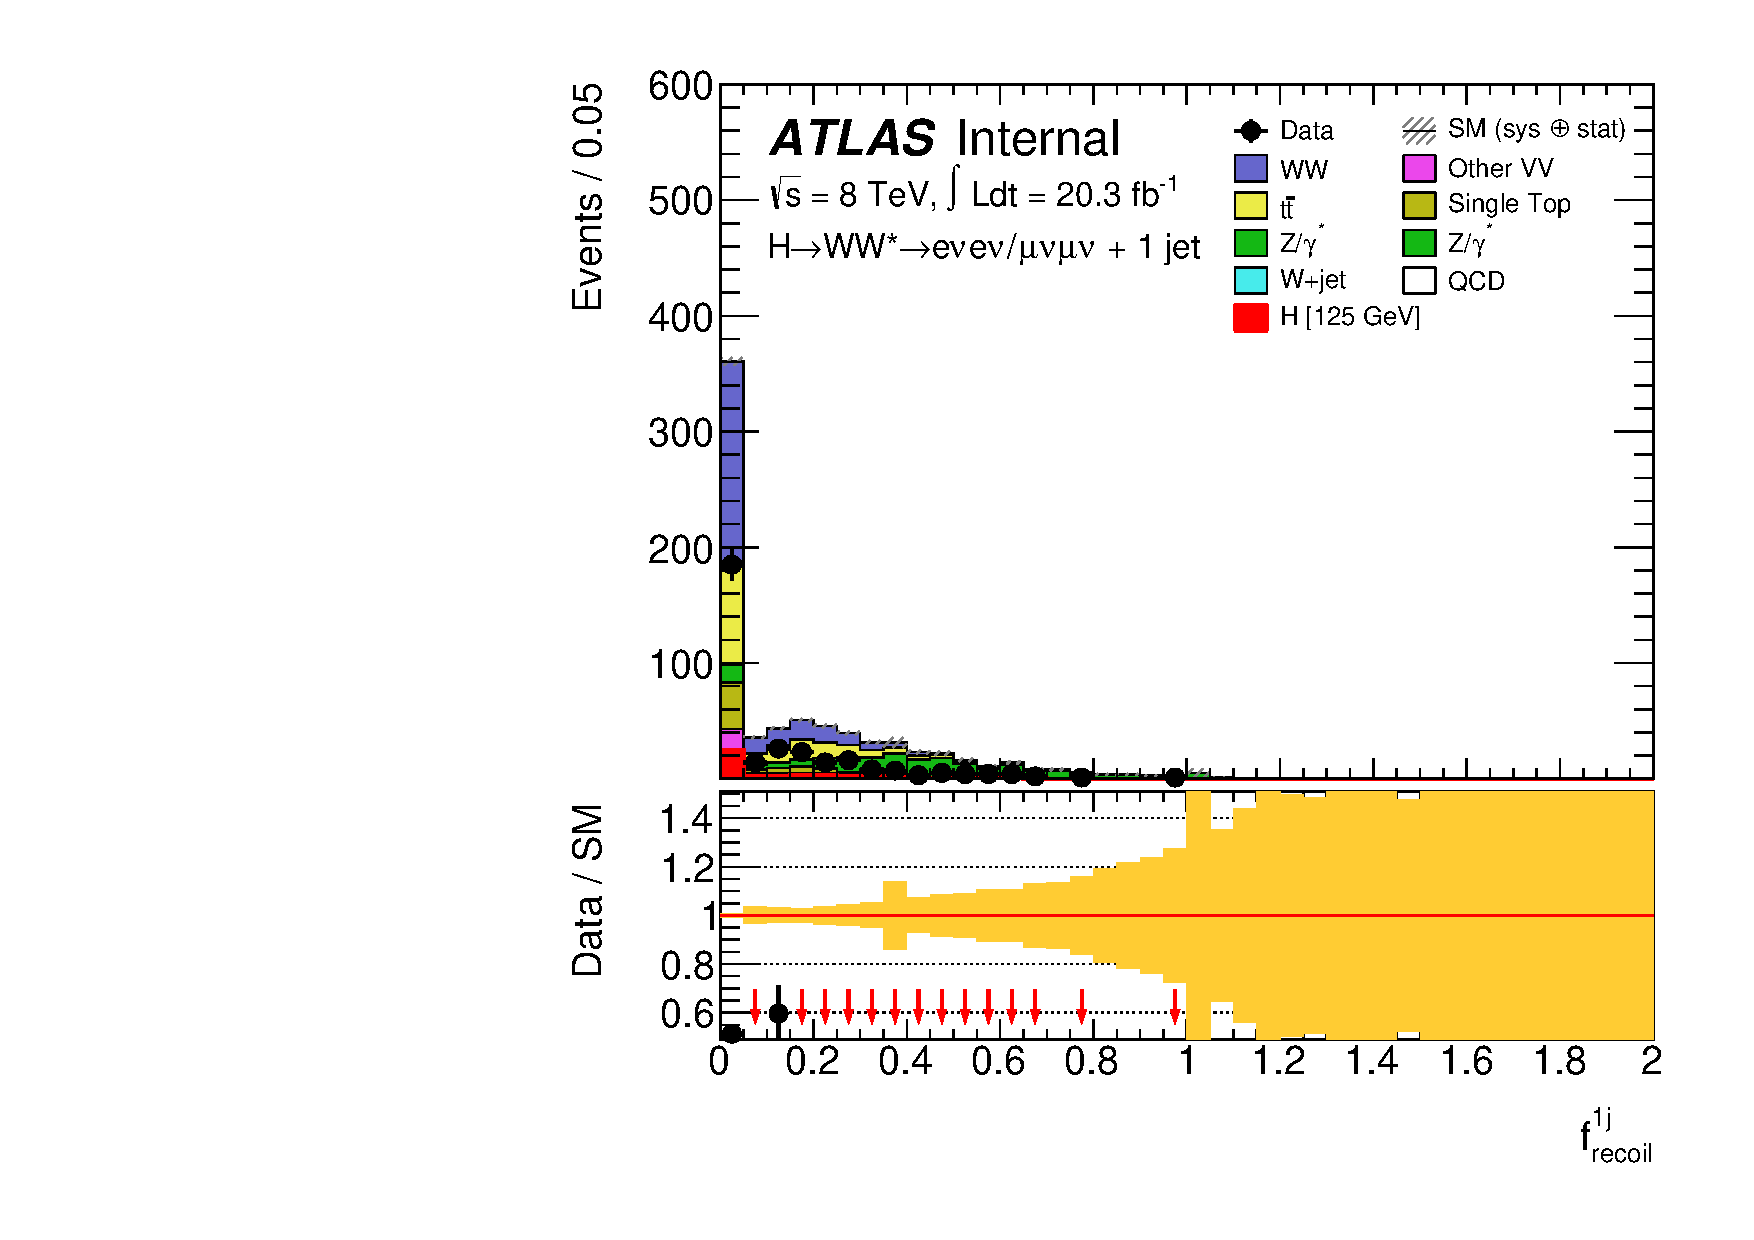
\includegraphics[width=0.495\textwidth]{tex/selection/eemm_CutTopoDPhill_1jet_f_recoil_ext_mh125_lin}
	\caption{The \corrtrackmetrel (left) and \frecoil (right) distributions directly 
	before they are cut upon in the \eech/\mmch channels.}
	\label{fig:sel:1j:sf_cuts}
\end{figure}

The event yields of the 1-jet selection are provided in \Appendix~\ref{app:sr_yields}, 
and the \mt distributions of the selected events are shown in \Figure~\ref{fig:sel:1j:mt}.

\begin{figure}
	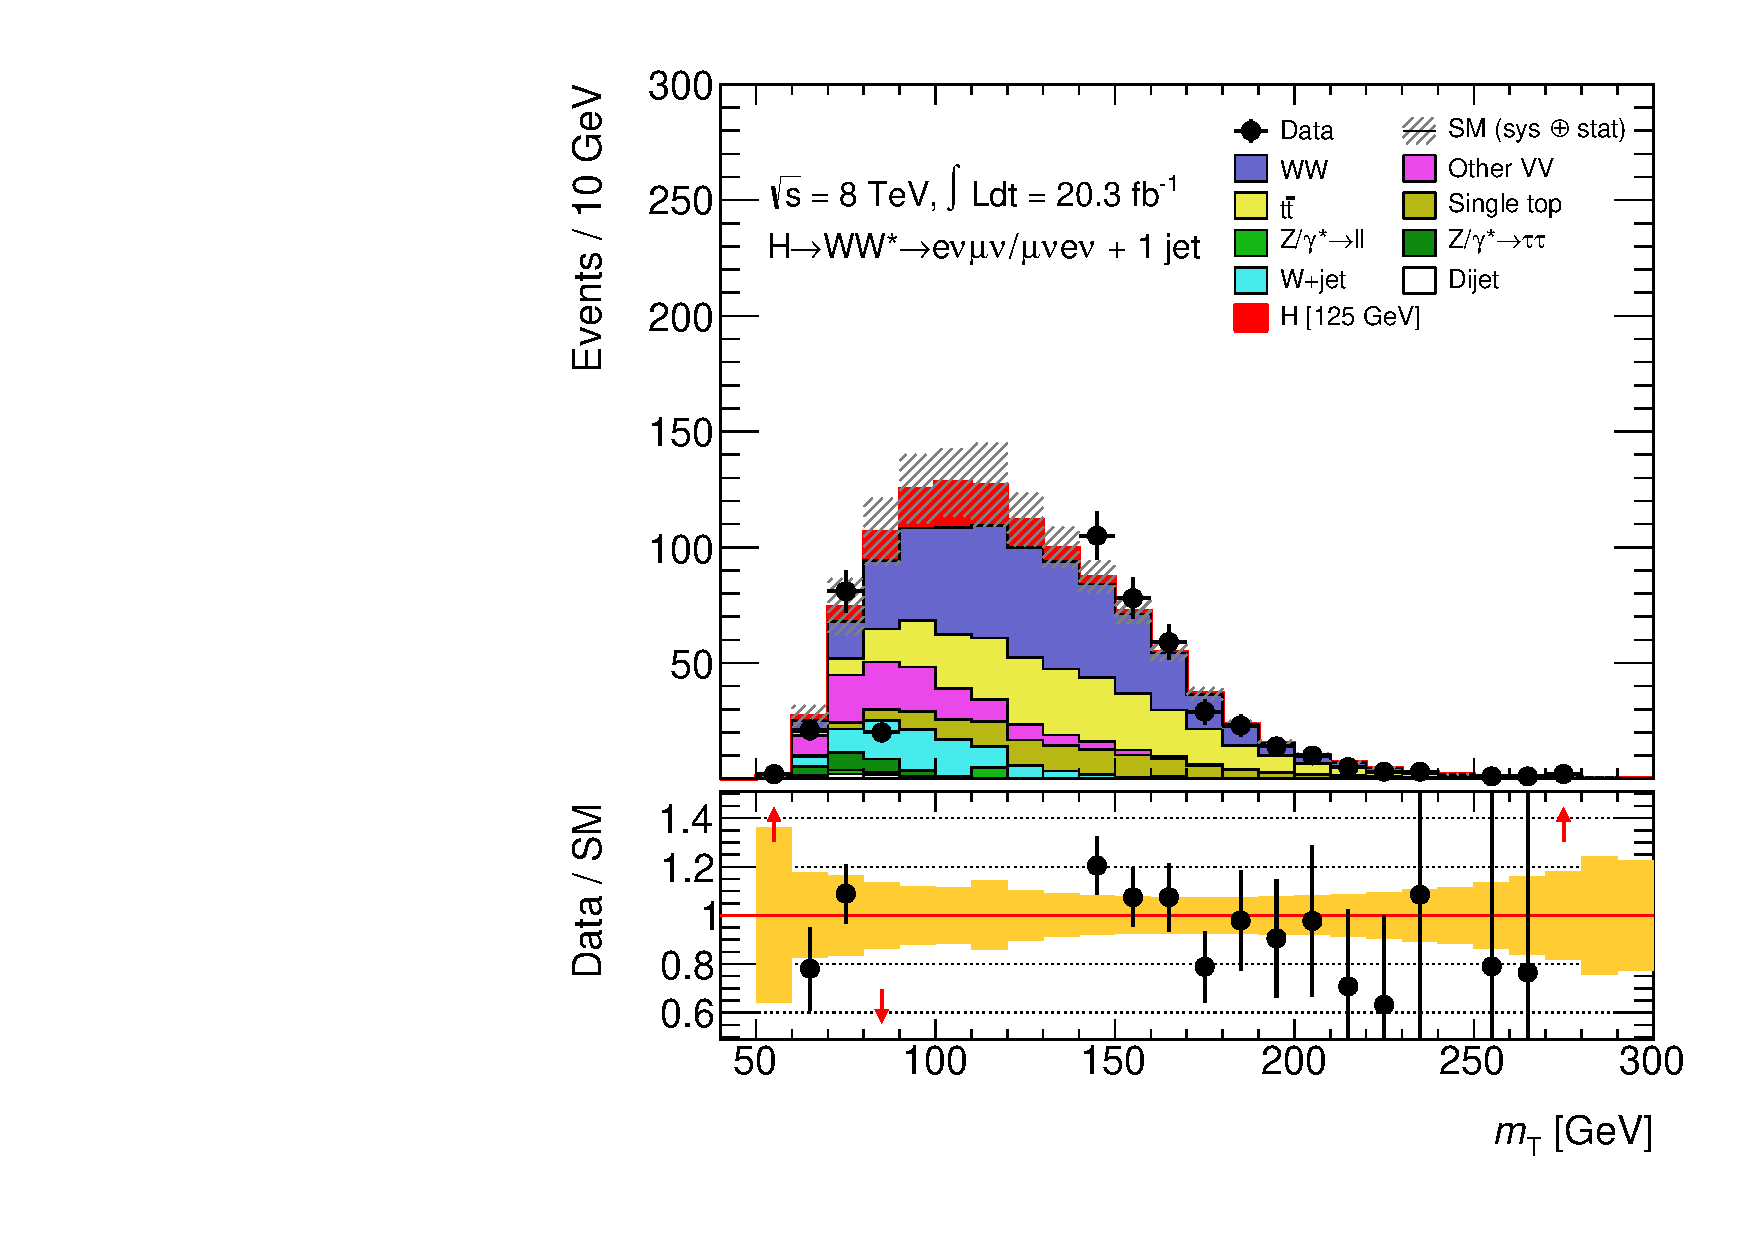
\includegraphics[width=0.495\textwidth]{tex/selection/emme_CutFRecoil_1jet_MT_TrackHWW_Clj_mh125_lin}
	\hfill
	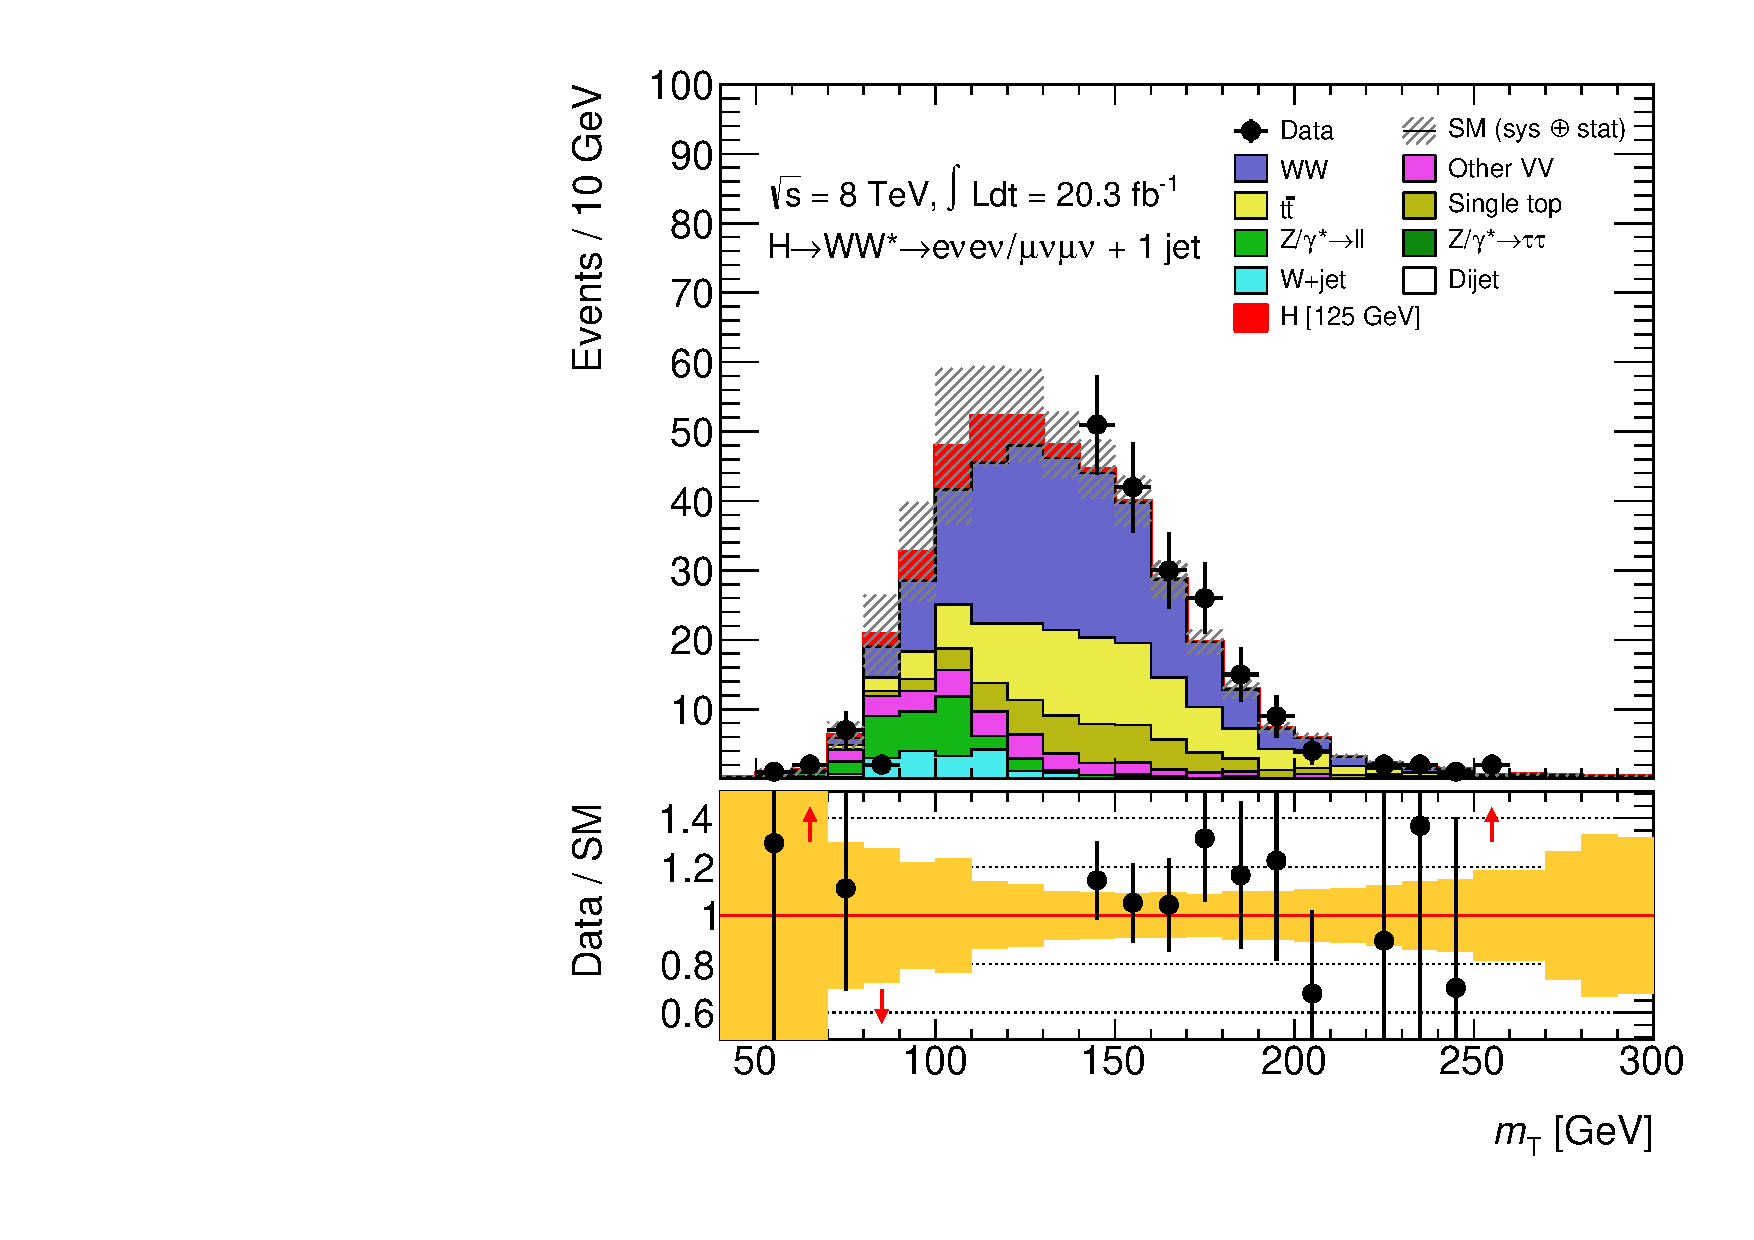
\includegraphics[width=0.495\textwidth]{tex/selection/eemm_CutFRecoil_1jet_MT_TrackHWW_Clj_mh125_lin}
	\caption{The \mt distribution of the selected 1-jet events, in the \emch/\mech (left) and 
	\eech/\mmch (right) channels.}
	\label{fig:sel:1j:mt}
\end{figure}



\subsection{\twojet selection}
\label{sec:selection:2j}

Only the \emch/\mech channels are used in the \twojet bin, which is dominated by top 
background (see \Figure~\ref{fig:sel:njets}). Note that variable definitions using only 
two jets refer to the two hardest jets. As in the 1-jet bin, the top background is 
greatly suppressed by vetoing events with a \Pbottom-tagged jet with 
\unit{$\pt > 20$}{\GeV}. Also, the \DYtt background is again suppressed by the 
requirement \unit{$\mtautau < \mZ - 25$}{\GeV}.

At this point, it is necessary to contextualise the analysis. Although this thesis 
describes the search for the ggF production mode, searches for the other production modes 
(see \Section~\ref{sec:properties}) are also performed by the ATLAS collaboration. To 
simplify the statistical combination of these searches, it is helpful to avoid overlap 
between their signal regions. This is particularly important for the \twojet bin.

The VBF production mode features two outgoing quarks at LO (see 
\Figure~\ref{fig:feyn:VBF}). 
Therefore the \twojet bin is the starting point for the VBF selection. However, the 
absence of colour exchange between the quarks leads to dramatically different event 
topologies compared to ggF events in the \twojet bin; VBF events feature two high-\pt 
jets, separated by a large rapidity gap devoid of hadronic activity. Thus, events 
containing a softer jet with \unit{$\pt > 20$}{\GeV} within this rapidity gap are removed 
from the VBF selection. This is the \textit{central jet veto} (CJV). The VBF selection 
also requires that the leptons lie within this rapidity gap, since the Higgs boson is 
generally produced centrally. This is the \textit{outside lepton veto} (OLV). Finally, a 
boosted decision tree (BDT) \cite{TMVA} is trained to discriminate VBF events based upon 
eight input variables:

\begin{listliketab}
	\begin{tabular}{Ll@{\hskip 0.3in}llll}
		\textbullet & VBF topology:    & \mjj, &\dyjj, &$\eta_{\Plepton}$ centrality, &$\sum_{\Plepton, j} m_{\Plepton j}$ \\
		\textbullet & \HWW decay:      & \mll, &\dphill, &\mt \\
		\textbullet & top suppression: & \pttot \\
	\end{tabular}
\end{listliketab}

\noindent
$\eta_{\Plepton}$ centrality characterises how close the leptons are to the jets. 
$\sum_{\Plepton, j} m_{\Plepton j}$ sums the masses of the four lepton-jet systems 
possible with the two hardest jets, which is higher in VBF events due to the large 
separations involved. \pttot is the sum of \corrtrackmetvec and the \ptvec of each lepton 
and jet, capturing the soft hadronic recoil, which is larger in top background events. 
The BDT scores events between 100\% signal-like ($+1$) and 100\% background-like ($-1$), 
where ggF is considered a background. Events with a score $> -0.48$ are selected (see 
\Figure~\todo{VBF BDT plot}).

Another search considers the \WH and \ZH production modes, where the vector boson decays 
hadronically (see \Figure~\ref{fig:feyn:VH}). Again, the \twojet bin is the starting 
point for this selection. As with VBF, the jet kinematics can be used to distinguish this 
from ggF. First, the criterion $\dyjj < 1.2$ requires small jet separation, since the 
vector boson is likely to be produced with significant momentum. Second, the di-jet 
system must have a mass corresponding to a \PW or \PZ boson, 
\unit{$\mods{\mjj - 85}$}{\GeV}.

To maintain orthogonality with the VBF and \VH analyses, the ggF analysis requires events 
in the \twojet bin to fail at least one cut from each selection. That is, an event must 
fail either the CJV, the OLV \textbf{or} the BDT score cut \textbf{and} it must fail 
either the \dyjj \textbf{or} the \mjj cut.



\subsection{Summary}
\label{sec:selection:summary}

The entire event selection is concisely summarised in \Table~\ref{tab:event_selection}. 
In total, there are 10 different signal regions: $\braces{\emch,\mech,\eech,\mmch} 
\otimes \braces{\text{0-jet,1-jet}} \oplus \braces{\emch,\mech} \otimes \twojet$. The 
events in these signal regions shall be input to the fitting procedure in 
\Chapter~\ref{chap:results}.

\begin{sidewaystable}
	\centering
	\begin{tabularx}{1.05\textwidth}{l *{6}{Y}}
		\toprule
		&&& \multicolumn{2}{c}{All jet bins} \\
		\cmidrule(lr){4-5}
		&&& \emch/\mech & \eech/\mmch \\
		\cmidrule(lr){2-7}
		\ldelim\{{3}{2.5cm}[Pre-selection] 
		& \multicolumn{6}{c}{$\ptleadlep > 22$ and $\ptsubleadlep > 10$} \\
		&&& $\mll > 12$ & $\mll > 10$ \\
		&&& -- & $\mods{\mll - \mZ} > 15$ \\ [1ex]
		\cmidrule(lr){2-7}
		&\multicolumn{2}{c}{0-jet bin} & \multicolumn{2}{c}{1-jet bin} & \multicolumn{2}{c}{\twojet bin} \\
		\cmidrule(lr){2-3} \cmidrule(lr){4-5} \cmidrule(lr){6-7}
		& \emch/\mech & \eech/\mmch & \emch/\mech & \eech/\mmch & \multicolumn{2}{c}{\emch/\mech} \\
		\cmidrule(lr){2-7}
		\ldelim\{{4}{2.5cm}[Reject \DY] 
		& $\corrtrackmet > 20$ & $\metrel > 40$ & $\corrtrackmet > 10$ & $\metrel > 40$ & \multicolumn{2}{c}{$\corrtrackmet > 20$} \\
		& \multicolumn{2}{c}{$\ptll > 30$} & $\mtautau < \mZ - 25$ & -- & \multicolumn{2}{c}{$\mtautau < \mZ - 25$} \\
		& -- & $\trackmetrel > 40$ & -- & $\trackmetrel > 35$ & \multicolumn{2}{c}{--} \\
		& -- & $\frecoil < 0.1$ & -- & $\frecoil < 0.1$ & \multicolumn{2}{c}{--} \\
		Reject fakes
		& \multicolumn{2}{c}{$\dphillmet > \pi/2$} & $\maxmtw > 50$ & -- & \multicolumn{2}{c}{--} \\
		Reject top 
		& \multicolumn{2}{c}{--} & \multicolumn{2}{c}{$\nbjets = 0$} & \multicolumn{2}{c}{$\nbjets = 0$} \\
		Reject VBF
		& \multicolumn{2}{c}{--} & \multicolumn{2}{c}{--} & \multicolumn{2}{c}{Fail CJV, OLV or BDT} \\
		Reject \VH
		& \multicolumn{2}{c}{--} & \multicolumn{2}{c}{--} & \multicolumn{2}{c}{Fail $\dyjj < 1.2$ or $\mods{\mjj - 85} < 15$} \\ [1ex]
		\cmidrule(lr){2-7}
		&&& \multicolumn{2}{c}{All jet bins} \\
		\cmidrule(lr){4-5}
		&&& \emch/\mech & \eech/\mmch \\
		\cmidrule(lr){2-7}
		\ldelim\{{2}{2.5cm}[Select signal]
		&&& \multicolumn{2}{c}{$\mll < 55$} \\
		&&& \multicolumn{2}{c}{$\dphill < 1.8$} \\
		\bottomrule
	\end{tabularx}
	\caption{Summary of ggF event selection. Cuts on energy, momentum and mass are given 
	in \GeV, and angular cuts are given in radians. The relevant variables are described 
	in the text.}
	\label{tab:event_selection}
\end{sidewaystable}


